\documentclass[twoside]{book}

% Packages required by doxygen
\usepackage{fixltx2e}
\usepackage{calc}
\usepackage{doxygen}
\usepackage{graphicx}
\usepackage[utf8]{inputenc}
\usepackage{makeidx}
\usepackage{multicol}
\usepackage{multirow}
\PassOptionsToPackage{warn}{textcomp}
\usepackage{textcomp}
\usepackage[nointegrals]{wasysym}
\usepackage[table]{xcolor}

% Font selection
\usepackage[T1]{fontenc}
\usepackage{mathptmx}
\usepackage[scaled=.90]{helvet}
\usepackage{courier}
\usepackage{amssymb}
\usepackage{sectsty}
\renewcommand{\familydefault}{\sfdefault}
\allsectionsfont{%
  \fontseries{bc}\selectfont%
  \color{darkgray}%
}
\renewcommand{\DoxyLabelFont}{%
  \fontseries{bc}\selectfont%
  \color{darkgray}%
}
\newcommand{\+}{\discretionary{\mbox{\scriptsize$\hookleftarrow$}}{}{}}

% Page & text layout
\usepackage{geometry}
\geometry{%
  a4paper,%
  top=2.5cm,%
  bottom=2.5cm,%
  left=2.5cm,%
  right=2.5cm%
}
\tolerance=750
\hfuzz=15pt
\hbadness=750
\setlength{\emergencystretch}{15pt}
\setlength{\parindent}{0cm}
\setlength{\parskip}{0.2cm}
\makeatletter
\renewcommand{\paragraph}{%
  \@startsection{paragraph}{4}{0ex}{-1.0ex}{1.0ex}{%
    \normalfont\normalsize\bfseries\SS@parafont%
  }%
}
\renewcommand{\subparagraph}{%
  \@startsection{subparagraph}{5}{0ex}{-1.0ex}{1.0ex}{%
    \normalfont\normalsize\bfseries\SS@subparafont%
  }%
}
\makeatother

% Headers & footers
\usepackage{fancyhdr}
\pagestyle{fancyplain}
\fancyhead[LE]{\fancyplain{}{\bfseries\thepage}}
\fancyhead[CE]{\fancyplain{}{}}
\fancyhead[RE]{\fancyplain{}{\bfseries\leftmark}}
\fancyhead[LO]{\fancyplain{}{\bfseries\rightmark}}
\fancyhead[CO]{\fancyplain{}{}}
\fancyhead[RO]{\fancyplain{}{\bfseries\thepage}}
\fancyfoot[LE]{\fancyplain{}{}}
\fancyfoot[CE]{\fancyplain{}{}}
\fancyfoot[RE]{\fancyplain{}{\bfseries\scriptsize 生成于 2014年 七月 22日 星期二 10\+:59\+:47 , 为 Rain P\+H\+P Framework(\+R\+P\+F)使用  Doxygen }}
\fancyfoot[LO]{\fancyplain{}{\bfseries\scriptsize 生成于 2014年 七月 22日 星期二 10\+:59\+:47 , 为 Rain P\+H\+P Framework(\+R\+P\+F)使用  Doxygen }}
\fancyfoot[CO]{\fancyplain{}{}}
\fancyfoot[RO]{\fancyplain{}{}}
\renewcommand{\footrulewidth}{0.4pt}
\renewcommand{\chaptermark}[1]{%
  \markboth{#1}{}%
}
\renewcommand{\sectionmark}[1]{%
  \markright{\thesection\ #1}%
}

% Indices & bibliography
\usepackage{natbib}
\usepackage[titles]{tocloft}
\setcounter{tocdepth}{3}
\setcounter{secnumdepth}{5}
\makeindex

% Hyperlinks (required, but should be loaded last)
\usepackage{ifpdf}
\ifpdf
  \usepackage[pdftex,pagebackref=true]{hyperref}
\else
  \usepackage[ps2pdf,pagebackref=true]{hyperref}
\fi
\hypersetup{%
  colorlinks=true,%
  linkcolor=blue,%
  citecolor=blue,%
  unicode%
}

% Custom commands
\newcommand{\clearemptydoublepage}{%
  \newpage{\pagestyle{empty}\cleardoublepage}%
}


%===== C O N T E N T S =====

\begin{document}

% Titlepage & ToC
\hypersetup{pageanchor=false,
             bookmarks=true,
             bookmarksnumbered=true,
             pdfencoding=unicode
            }
\pagenumbering{roman}
\begin{titlepage}
\vspace*{7cm}
\begin{center}%
{\Large Rain P\+H\+P Framework(R\+P\+F) \\[1ex]\large 0.\+1.\+1 }\\
\vspace*{1cm}
{\large 制作者 Doxygen 1.8.7}\\
\vspace*{0.5cm}
{\small 2014年 七月 22日 星期二 10:59:47}\\
\end{center}
\end{titlepage}
\clearemptydoublepage
\tableofcontents
\clearemptydoublepage
\pagenumbering{arabic}
\hypersetup{pageanchor=true}

%--- Begin generated contents ---
\chapter{待办事项列表}
\label{todo}
\hypertarget{todo}{}

\begin{DoxyRefList}
\item[\label{todo__todo000001}%
\hypertarget{todo__todo000001}{}%
成员 \hyperlink{classPHPMailer_ad7dfabb6c5e91e298be2de2e78749a75}{P\+H\+P\+Mailer\+:\+:set} (\$name, \$value= '')]Should this not be using \+\_\+\+\_\+set() magic function? 
\end{DoxyRefList}
\chapter{命名空间索引}
\section{命名空间列表}
这里列出了所有文档化的命名空间定义,附带简要说明\+:\begin{DoxyCompactList}
\item\contentsline{section}{\hyperlink{namespacePHPMailer}{P\+H\+P\+Mailer} }{\pageref{namespacePHPMailer}}{}
\end{DoxyCompactList}

\chapter{继承关系索引}
\section{类继承关系}
此继承关系列表按字典顺序粗略的排序\+: \begin{DoxyCompactList}
\item \contentsline{section}{Action}{\pageref{classAction}}{}
\item \contentsline{section}{Cache}{\pageref{classCache}}{}
\item \contentsline{section}{Config}{\pageref{classConfig}}{}
\item \contentsline{section}{Controller}{\pageref{classController}}{}
\item \contentsline{section}{Demo}{\pageref{classDemo}}{}
\item Exception\begin{DoxyCompactList}
\item \contentsline{section}{phpmailer\+Exception}{\pageref{classphpmailerException}}{}
\end{DoxyCompactList}
\item \contentsline{section}{Ftp}{\pageref{classFtp}}{}
\item \contentsline{section}{Image}{\pageref{classImage}}{}
\item \contentsline{section}{Kernel}{\pageref{classKernel}}{}
\item \contentsline{section}{Lang}{\pageref{classLang}}{}
\item \contentsline{section}{Model}{\pageref{classModel}}{}
\item \contentsline{section}{Mysql}{\pageref{classMysql}}{}
\item \contentsline{section}{Page}{\pageref{classPage}}{}
\item \contentsline{section}{P\+H\+P\+Mailer}{\pageref{classPHPMailer}}{}
\item \contentsline{section}{Session}{\pageref{classSession}}{}
\item \contentsline{section}{S\+M\+T\+P}{\pageref{classSMTP}}{}
\item \contentsline{section}{Upload}{\pageref{classUpload}}{}
\end{DoxyCompactList}

\chapter{类索引}
\section{类列表}
这里列出了所有类、结构、联合以及接口定义等,并附带简要说明\+:\begin{DoxyCompactList}
\item\contentsline{section}{\hyperlink{classAction}{Action} }{\pageref{classAction}}{}
\item\contentsline{section}{\hyperlink{classCache}{Cache} }{\pageref{classCache}}{}
\item\contentsline{section}{\hyperlink{classConfig}{Config} }{\pageref{classConfig}}{}
\item\contentsline{section}{\hyperlink{classController}{Controller} }{\pageref{classController}}{}
\item\contentsline{section}{\hyperlink{classDemo}{Demo} }{\pageref{classDemo}}{}
\item\contentsline{section}{\hyperlink{classFtp}{Ftp} }{\pageref{classFtp}}{}
\item\contentsline{section}{\hyperlink{classImage}{Image} }{\pageref{classImage}}{}
\item\contentsline{section}{\hyperlink{classKernel}{Kernel} }{\pageref{classKernel}}{}
\item\contentsline{section}{\hyperlink{classLang}{Lang} }{\pageref{classLang}}{}
\item\contentsline{section}{\hyperlink{classModel}{Model} }{\pageref{classModel}}{}
\item\contentsline{section}{\hyperlink{classMysql}{Mysql} }{\pageref{classMysql}}{}
\item\contentsline{section}{\hyperlink{classPage}{Page} }{\pageref{classPage}}{}
\item\contentsline{section}{\hyperlink{classPHPMailer}{P\+H\+P\+Mailer} }{\pageref{classPHPMailer}}{}
\item\contentsline{section}{\hyperlink{classphpmailerException}{phpmailer\+Exception} }{\pageref{classphpmailerException}}{}
\item\contentsline{section}{\hyperlink{classSession}{Session} }{\pageref{classSession}}{}
\item\contentsline{section}{\hyperlink{classSMTP}{S\+M\+T\+P} }{\pageref{classSMTP}}{}
\item\contentsline{section}{\hyperlink{classUpload}{Upload} }{\pageref{classUpload}}{}
\end{DoxyCompactList}

\chapter{命名空间文档}
\hypertarget{namespacePHPMailer}{\section{P\+H\+P\+Mailer 命名空间参考}
\label{namespacePHPMailer}\index{P\+H\+P\+Mailer@{P\+H\+P\+Mailer}}
}


\subsection{详细描述}
\hyperlink{classPHPMailer}{P\+H\+P\+Mailer} -\/ P\+H\+P email transport class N\+O\+T\+E\+: Requires P\+H\+P version 5 or later

\begin{DoxyAuthor}{作者}
Andy Prevost 

Marcus Bointon 
\end{DoxyAuthor}
\begin{DoxyCopyright}{版权所有}
2004 -\/ 2009 Andy Prevost 
\end{DoxyCopyright}
\begin{DoxyVersion}{版本}

\end{DoxyVersion}
\begin{DoxyParagraph}{Id}
class.\+phpmailer.\+php 447 2009-\/05-\/25 01\+:36\+:38\+Z codeworxtech 
\end{DoxyParagraph}
\href{http://www.gnu.org/copyleft/lesser.html}{\tt http\+://www.\+gnu.\+org/copyleft/lesser.\+html} G\+N\+U Lesser General Public License

\hyperlink{classPHPMailer}{P\+H\+P\+Mailer} -\/ P\+H\+P \hyperlink{classSMTP}{S\+M\+T\+P} email transport class N\+O\+T\+E\+: Designed for use with P\+H\+P version 5 and up

\begin{DoxyAuthor}{作者}
Andy Prevost 

Marcus Bointon 
\end{DoxyAuthor}
\begin{DoxyCopyright}{版权所有}
2004 -\/ 2008 Andy Prevost  \href{http://www.gnu.org/copyleft/lesser.html}{\tt http\+://www.\+gnu.\+org/copyleft/lesser.\+html} Distributed under the Lesser General Public License (L\+G\+P\+L) 
\end{DoxyCopyright}
\begin{DoxyVersion}{版本}

\end{DoxyVersion}
\begin{DoxyParagraph}{Id}
class.\+smtp.\+php 444 2009-\/05-\/05 11\+:22\+:26\+Z coolbru 
\end{DoxyParagraph}

\chapter{类说明}
\hypertarget{classAction}{\section{Action类 参考}
\label{classAction}\index{Action@{Action}}
}
\subsection*{Protected 成员函数}
\begin{DoxyCompactItemize}
\item 
\hypertarget{classAction_a36e0fbe39840e8713aa5e57c6ec77525}{{\bfseries init} ()}\label{classAction_a36e0fbe39840e8713aa5e57c6ec77525}

\item 
\hypertarget{classAction_a89048985af4d911c73c9b3582eaac0db}{{\bfseries success} (\$msg= '操作成功', \$code=200, \$nav\+Tab\+Id= '', \$rel= '', \$callback\+Type= '', \$forward\+Url= '', \$confirm\+Msg= '')}\label{classAction_a89048985af4d911c73c9b3582eaac0db}

\item 
\hypertarget{classAction_add0871e8a54f41233a4a442a18eed77f}{{\bfseries error} (\$msg= '操作失败', \$code=300, \$nav\+Tab\+Id= '', \$rel= '', \$callback\+Type= '', \$forward\+Url= '', \$confirm\+Msg= '')}\label{classAction_add0871e8a54f41233a4a442a18eed77f}

\item 
\hypertarget{classAction_a70704095c8d66340022d227d99470649}{{\bfseries timeout} (\$msg= '操作超时', \$code=301, \$nav\+Tab\+Id= '', \$rel= '', \$callback\+Type= '', \$forward\+Url= '', \$confirm\+Msg= '')}\label{classAction_a70704095c8d66340022d227d99470649}

\item 
\hypertarget{classAction_a3a56b1c959956b671038c1f8bcd6dfb4}{{\bfseries run} ()}\label{classAction_a3a56b1c959956b671038c1f8bcd6dfb4}

\item 
\hypertarget{classAction_a393ee8679b3bdf2db1571882247e2686}{{\bfseries checktoken} ()}\label{classAction_a393ee8679b3bdf2db1571882247e2686}

\item 
\hypertarget{classAction_a14514e26573354d09824c35251155d88}{{\bfseries set} (\$key, \$val)}\label{classAction_a14514e26573354d09824c35251155d88}

\item 
\hypertarget{classAction_ab80a2d32134ea0e91f516c74a0eae0f3}{{\bfseries display} (\$tpl=null)}\label{classAction_ab80a2d32134ea0e91f516c74a0eae0f3}

\end{DoxyCompactItemize}
\subsection*{Protected 属性}
\begin{DoxyCompactItemize}
\item 
\hypertarget{classAction_a605a5c8f27fefd824144f7b7a45c6e96}{{\bfseries \$open\+\_\+token} = true}\label{classAction_a605a5c8f27fefd824144f7b7a45c6e96}

\end{DoxyCompactItemize}


\subsection{详细描述}
所有的action都应该继承此类 

该类的文档由以下文件生成\+:\begin{DoxyCompactItemize}
\item 
framework/kernel/Action.\+class.\+php\end{DoxyCompactItemize}

\hypertarget{classCache}{\section{Cache类 参考}
\label{classCache}\index{Cache@{Cache}}
}
\subsection*{Public 成员函数}
\begin{DoxyCompactItemize}
\item 
\hypertarget{classCache_a81f7747d3dd8a544d3cc20177483bfd2}{{\bfseries connect} ()}\label{classCache_a81f7747d3dd8a544d3cc20177483bfd2}

\item 
\hypertarget{classCache_a88748cfd9005e9dd8179c6774ea1378b}{{\bfseries clear} ()}\label{classCache_a88748cfd9005e9dd8179c6774ea1378b}

\item 
\hypertarget{classCache_ad25f006b5b60f18f23b3009ed18ce35b}{{\bfseries get} (\$key)}\label{classCache_ad25f006b5b60f18f23b3009ed18ce35b}

\item 
\hypertarget{classCache_a4bb2d39b510c73dce7a0740906226329}{{\bfseries rm} (\$key)}\label{classCache_a4bb2d39b510c73dce7a0740906226329}

\item 
\hypertarget{classCache_aca221ddf7cf4f4e26c0aa1ae38cd069f}{{\bfseries set} (\$key, \$val, \$expire=1200)}\label{classCache_aca221ddf7cf4f4e26c0aa1ae38cd069f}

\item 
\hypertarget{classCache_aebd1c49aa2b47c34f8af6b688a6922d4}{{\bfseries free} ()}\label{classCache_aebd1c49aa2b47c34f8af6b688a6922d4}

\end{DoxyCompactItemize}
\subsection*{静态 Public 成员函数}
\begin{DoxyCompactItemize}
\item 
\hypertarget{classCache_a1c8b6e18a6cf407216f4f7f7f3fefe7f}{static {\bfseries get\+Instance} (\$type= 'f', \$conf=null)}\label{classCache_a1c8b6e18a6cf407216f4f7f7f3fefe7f}

\end{DoxyCompactItemize}


该类的文档由以下文件生成\+:\begin{DoxyCompactItemize}
\item 
framework/lib/core/Cache.\+class.\+php\end{DoxyCompactItemize}

\hypertarget{classConfig}{\section{Config类 参考}
\label{classConfig}\index{Config@{Config}}
}
\subsection*{静态 Public 成员函数}
\begin{DoxyCompactItemize}
\item 
\hypertarget{classConfig_a6849a4afeb4cf7e3905861933824cd59}{static {\bfseries set} (\$key, \$val)}\label{classConfig_a6849a4afeb4cf7e3905861933824cd59}

\item 
\hypertarget{classConfig_a31827e08ef05915e5cbe9fab4dbb283b}{static {\bfseries get} (\$key)}\label{classConfig_a31827e08ef05915e5cbe9fab4dbb283b}

\item 
\hypertarget{classConfig_ab4abf94b1b9efc4c85187cd4b256a80b}{static {\bfseries rm} (\$key)}\label{classConfig_ab4abf94b1b9efc4c85187cd4b256a80b}

\item 
\hypertarget{classConfig_a9b8aeccd062cd33d37b8f90dd4b4c6d5}{static {\bfseries exist} (\$key)}\label{classConfig_a9b8aeccd062cd33d37b8f90dd4b4c6d5}

\end{DoxyCompactItemize}


该类的文档由以下文件生成\+:\begin{DoxyCompactItemize}
\item 
framework/kernel/Config.\+class.\+php\end{DoxyCompactItemize}

\hypertarget{classController}{\section{Controller类 参考}
\label{classController}\index{Controller@{Controller}}
}
\subsection*{Protected 成员函数}
\begin{DoxyCompactItemize}
\item 
\hypertarget{classController_af71b414389f649229743b8e8b16e1ee8}{{\bfseries init} ()}\label{classController_af71b414389f649229743b8e8b16e1ee8}

\end{DoxyCompactItemize}


该类的文档由以下文件生成\+:\begin{DoxyCompactItemize}
\item 
framework/kernel/Controller.\+class.\+php\end{DoxyCompactItemize}

\hypertarget{classDemo}{\section{Demo类 参考}
\label{classDemo}\index{Demo@{Demo}}
}
\subsection*{静态 Public 成员函数}
\begin{DoxyCompactItemize}
\item 
\hypertarget{classDemo_a1f054c304228ce0b56da3195955ce6a6}{static {\bfseries cdemo} ()}\label{classDemo_a1f054c304228ce0b56da3195955ce6a6}

\end{DoxyCompactItemize}


该类的文档由以下文件生成\+:\begin{DoxyCompactItemize}
\item 
framework/lib/core/Demo.\+class.\+php\end{DoxyCompactItemize}

\hypertarget{classFtp}{\section{Ftp类 参考}
\label{classFtp}\index{Ftp@{Ftp}}
}
\subsection*{Public 成员函数}
\begin{DoxyCompactItemize}
\item 
\hyperlink{classFtp_a6e16a450ba38e9cf178b13ff3e091443}{\+\_\+\+\_\+construct} (\$config=array())
\item 
\hyperlink{classFtp_acbe05ba238542a10c1b0623ecf7d2081}{connect} (\$config=array())
\item 
\hyperlink{classFtp_aade650c29b7b10938c1dd32842cc43f2}{chgdir} (\$path= '', \$supress\+\_\+debug=F\+A\+L\+S\+E)
\item 
\hyperlink{classFtp_ae876a655c13c8418289e5f6751a0b2f1}{mkdir} (\$path= '', \$permissions=N\+U\+L\+L)
\item 
\hyperlink{classFtp_aae84f09cc3a13e23a78e68a91638717e}{upload} (\$localpath, \$remotepath, \$mode= 'auto', \$permissions=N\+U\+L\+L)
\item 
\hyperlink{classFtp_a4c03629438e7c033e09940f14feae8b4}{download} (\$remotepath, \$localpath, \$mode= 'auto')
\item 
\hyperlink{classFtp_a25301a57eceb2091105c29835687c461}{rename} (\$oldname, \$newname, \$move=F\+A\+L\+S\+E)
\item 
\hyperlink{classFtp_a2887ad771ff19eaa0041f8e9db7dfbff}{delete\+\_\+file} (\$file)
\item 
\hyperlink{classFtp_a228bb4211ff78dc6bf6233f528bfffb0}{delete\+\_\+dir} (\$path)
\item 
\hyperlink{classFtp_a8b56d6b41df6e5adc6f68aaec73a8c3e}{chmod} (\$path, \$perm)
\item 
\hyperlink{classFtp_a9f23eba3ee61a3986a872d4f3665afec}{filelist} (\$path= '.')
\item 
\hyperlink{classFtp_a763b8546df21e02e9ead949e4e701803}{close} ()
\end{DoxyCompactItemize}


\subsection{详细描述}
仿写\+Code\+Igniter的\+F\+T\+P类 F\+T\+P基本操作: 1) 登陆; connect 2) 当前目录文件列表; filelist 3) 目录改变; chgdir 4) 重命名/移动; rename 5) 创建文件夹; mkdir 6) 删除; delete\+\_\+dir/delete\+\_\+file 7) 上传; upload 8) 下载 download

\begin{DoxyAuthor}{作者}
quanshuidingdang 
\end{DoxyAuthor}


\subsection{构造及析构函数说明}
\hypertarget{classFtp_a6e16a450ba38e9cf178b13ff3e091443}{\index{Ftp@{Ftp}!\+\_\+\+\_\+construct@{\+\_\+\+\_\+construct}}
\index{\+\_\+\+\_\+construct@{\+\_\+\+\_\+construct}!Ftp@{Ftp}}
\subsubsection[{\+\_\+\+\_\+construct}]{\setlength{\rightskip}{0pt plus 5cm}Ftp\+::\+\_\+\+\_\+construct (
\begin{DoxyParamCaption}
\item[{}]{\$config = {\ttfamily array()}}
\end{DoxyParamCaption}
)}}\label{classFtp_a6e16a450ba38e9cf178b13ff3e091443}
构造函数


\begin{DoxyParams}{参数}
{\em array} & 配置数组 \+: \$config = array('hostname'=$>$'','username'=$>$'','password'=$>$'','port'=$>$''...); \\
\hline
\end{DoxyParams}


\subsection{成员函数说明}
\hypertarget{classFtp_aade650c29b7b10938c1dd32842cc43f2}{\index{Ftp@{Ftp}!chgdir@{chgdir}}
\index{chgdir@{chgdir}!Ftp@{Ftp}}
\subsubsection[{chgdir}]{\setlength{\rightskip}{0pt plus 5cm}Ftp\+::chgdir (
\begin{DoxyParamCaption}
\item[{}]{\$path = {\ttfamily ''}, }
\item[{}]{\$supress\+\_\+debug = {\ttfamily FALSE}}
\end{DoxyParamCaption}
)}}\label{classFtp_aade650c29b7b10938c1dd32842cc43f2}
目录改变

public 
\begin{DoxyParams}{参数}
{\em string} & 目录标识(ftp) \\
\hline
{\em boolean} & \\
\hline
\end{DoxyParams}
\begin{DoxyReturn}{返回}
boolean 
\end{DoxyReturn}
\hypertarget{classFtp_a8b56d6b41df6e5adc6f68aaec73a8c3e}{\index{Ftp@{Ftp}!chmod@{chmod}}
\index{chmod@{chmod}!Ftp@{Ftp}}
\subsubsection[{chmod}]{\setlength{\rightskip}{0pt plus 5cm}Ftp\+::chmod (
\begin{DoxyParamCaption}
\item[{}]{\$path, }
\item[{}]{\$perm}
\end{DoxyParamCaption}
)}}\label{classFtp_a8b56d6b41df6e5adc6f68aaec73a8c3e}
修改文件权限

public 
\begin{DoxyParams}{参数}
{\em string} & 目录标识(ftp) \\
\hline
\end{DoxyParams}
\begin{DoxyReturn}{返回}
boolean 
\end{DoxyReturn}


参考自 mkdir() , 以及 upload().

\hypertarget{classFtp_a763b8546df21e02e9ead949e4e701803}{\index{Ftp@{Ftp}!close@{close}}
\index{close@{close}!Ftp@{Ftp}}
\subsubsection[{close}]{\setlength{\rightskip}{0pt plus 5cm}Ftp\+::close (
\begin{DoxyParamCaption}
{}
\end{DoxyParamCaption}
)}}\label{classFtp_a763b8546df21e02e9ead949e4e701803}
关闭\+F\+T\+P

public \begin{DoxyReturn}{返回}
boolean 
\end{DoxyReturn}
\hypertarget{classFtp_acbe05ba238542a10c1b0623ecf7d2081}{\index{Ftp@{Ftp}!connect@{connect}}
\index{connect@{connect}!Ftp@{Ftp}}
\subsubsection[{connect}]{\setlength{\rightskip}{0pt plus 5cm}Ftp\+::connect (
\begin{DoxyParamCaption}
\item[{}]{\$config = {\ttfamily array()}}
\end{DoxyParamCaption}
)}}\label{classFtp_acbe05ba238542a10c1b0623ecf7d2081}
F\+T\+P连接

public 
\begin{DoxyParams}{参数}
{\em array} & 配置数组 \\
\hline
\end{DoxyParams}
\begin{DoxyReturn}{返回}
boolean 
\end{DoxyReturn}
\hypertarget{classFtp_a228bb4211ff78dc6bf6233f528bfffb0}{\index{Ftp@{Ftp}!delete\+\_\+dir@{delete\+\_\+dir}}
\index{delete\+\_\+dir@{delete\+\_\+dir}!Ftp@{Ftp}}
\subsubsection[{delete\+\_\+dir}]{\setlength{\rightskip}{0pt plus 5cm}Ftp\+::delete\+\_\+dir (
\begin{DoxyParamCaption}
\item[{}]{\$path}
\end{DoxyParamCaption}
)}}\label{classFtp_a228bb4211ff78dc6bf6233f528bfffb0}
删除文件夹

public 
\begin{DoxyParams}{参数}
{\em string} & 目录标识(ftp) \\
\hline
\end{DoxyParams}
\begin{DoxyReturn}{返回}
boolean 
\end{DoxyReturn}
\hypertarget{classFtp_a2887ad771ff19eaa0041f8e9db7dfbff}{\index{Ftp@{Ftp}!delete\+\_\+file@{delete\+\_\+file}}
\index{delete\+\_\+file@{delete\+\_\+file}!Ftp@{Ftp}}
\subsubsection[{delete\+\_\+file}]{\setlength{\rightskip}{0pt plus 5cm}Ftp\+::delete\+\_\+file (
\begin{DoxyParamCaption}
\item[{}]{\$file}
\end{DoxyParamCaption}
)}}\label{classFtp_a2887ad771ff19eaa0041f8e9db7dfbff}
删除文件

public 
\begin{DoxyParams}{参数}
{\em string} & 文件标识(ftp) \\
\hline
\end{DoxyParams}
\begin{DoxyReturn}{返回}
boolean 
\end{DoxyReturn}


参考自 delete\+\_\+dir().

\hypertarget{classFtp_a4c03629438e7c033e09940f14feae8b4}{\index{Ftp@{Ftp}!download@{download}}
\index{download@{download}!Ftp@{Ftp}}
\subsubsection[{download}]{\setlength{\rightskip}{0pt plus 5cm}Ftp\+::download (
\begin{DoxyParamCaption}
\item[{}]{\$remotepath, }
\item[{}]{\$localpath, }
\item[{}]{\$mode = {\ttfamily 'auto'}}
\end{DoxyParamCaption}
)}}\label{classFtp_a4c03629438e7c033e09940f14feae8b4}
下载

public 
\begin{DoxyParams}{参数}
{\em string} & 远程目录标识(ftp) \\
\hline
{\em string} & 本地目录标识 \\
\hline
{\em string} & 下载模式 auto $\vert$$\vert$ ascii \\
\hline
\end{DoxyParams}
\begin{DoxyReturn}{返回}
boolean 
\end{DoxyReturn}
\hypertarget{classFtp_a9f23eba3ee61a3986a872d4f3665afec}{\index{Ftp@{Ftp}!filelist@{filelist}}
\index{filelist@{filelist}!Ftp@{Ftp}}
\subsubsection[{filelist}]{\setlength{\rightskip}{0pt plus 5cm}Ftp\+::filelist (
\begin{DoxyParamCaption}
\item[{}]{\$path = {\ttfamily '.'}}
\end{DoxyParamCaption}
)}}\label{classFtp_a9f23eba3ee61a3986a872d4f3665afec}
获取目录文件列表

public 
\begin{DoxyParams}{参数}
{\em string} & 目录标识(ftp) \\
\hline
\end{DoxyParams}
\begin{DoxyReturn}{返回}
array 
\end{DoxyReturn}


参考自 delete\+\_\+dir().

\hypertarget{classFtp_ae876a655c13c8418289e5f6751a0b2f1}{\index{Ftp@{Ftp}!mkdir@{mkdir}}
\index{mkdir@{mkdir}!Ftp@{Ftp}}
\subsubsection[{mkdir}]{\setlength{\rightskip}{0pt plus 5cm}Ftp\+::mkdir (
\begin{DoxyParamCaption}
\item[{}]{\$path = {\ttfamily ''}, }
\item[{}]{\$permissions = {\ttfamily NULL}}
\end{DoxyParamCaption}
)}}\label{classFtp_ae876a655c13c8418289e5f6751a0b2f1}
目录生成

public 
\begin{DoxyParams}{参数}
{\em string} & 目录标识(ftp) \\
\hline
{\em int} & 文件权限列表 \\
\hline
\end{DoxyParams}
\begin{DoxyReturn}{返回}
boolean 
\end{DoxyReturn}
\hypertarget{classFtp_a25301a57eceb2091105c29835687c461}{\index{Ftp@{Ftp}!rename@{rename}}
\index{rename@{rename}!Ftp@{Ftp}}
\subsubsection[{rename}]{\setlength{\rightskip}{0pt plus 5cm}Ftp\+::rename (
\begin{DoxyParamCaption}
\item[{}]{\$oldname, }
\item[{}]{\$newname, }
\item[{}]{\$move = {\ttfamily FALSE}}
\end{DoxyParamCaption}
)}}\label{classFtp_a25301a57eceb2091105c29835687c461}
重命名/移动

public 
\begin{DoxyParams}{参数}
{\em string} & 远程目录标识(ftp) \\
\hline
{\em string} & 新目录标识 \\
\hline
{\em boolean} & 判断是重命名(\+F\+A\+L\+S\+E)还是移动(\+T\+R\+U\+E) \\
\hline
\end{DoxyParams}
\begin{DoxyReturn}{返回}
boolean 
\end{DoxyReturn}
\hypertarget{classFtp_aae84f09cc3a13e23a78e68a91638717e}{\index{Ftp@{Ftp}!upload@{upload}}
\index{upload@{upload}!Ftp@{Ftp}}
\subsubsection[{upload}]{\setlength{\rightskip}{0pt plus 5cm}Ftp\+::upload (
\begin{DoxyParamCaption}
\item[{}]{\$localpath, }
\item[{}]{\$remotepath, }
\item[{}]{\$mode = {\ttfamily 'auto'}, }
\item[{}]{\$permissions = {\ttfamily NULL}}
\end{DoxyParamCaption}
)}}\label{classFtp_aae84f09cc3a13e23a78e68a91638717e}
上传

public 
\begin{DoxyParams}{参数}
{\em string} & 本地目录标识 \\
\hline
{\em string} & 远程目录标识(ftp) \\
\hline
{\em string} & 上传模式 auto $\vert$$\vert$ ascii \\
\hline
{\em int} & 上传后的文件权限列表 \\
\hline
\end{DoxyParams}
\begin{DoxyReturn}{返回}
boolean 
\end{DoxyReturn}


该类的文档由以下文件生成\+:\begin{DoxyCompactItemize}
\item 
framework/lib/vendor/ftp/Ftp.\+class.\+php\end{DoxyCompactItemize}

\hypertarget{classImage}{\section{Image类 参考}
\label{classImage}\index{Image@{Image}}
}
\subsection*{静态 Public 成员函数}
\begin{DoxyCompactItemize}
\item 
\hypertarget{classImage_ad665b63aa87b072bd796b20c30b0152e}{static {\bfseries get\+Code} (\$width=70, \$height=24, \$len=4)}\label{classImage_ad665b63aa87b072bd796b20c30b0152e}

\item 
\hypertarget{classImage_a87a55fa2f4340ef86598776b4f13dc32}{static {\bfseries image\+Water\+Mark} (\$ground\+Image, \$water\+Pos=0, \$water\+Image=\char`\"{}\char`\"{}, \$water\+Text=\char`\"{}\char`\"{}, \$font\+Size=12, \$text\+Color=\char`\"{}\#C\+C\+C\+C\+C\+C\char`\"{}, \$fontfile=null, \$x\+Offset=0, \$y\+Offset=0)}\label{classImage_a87a55fa2f4340ef86598776b4f13dc32}

\item 
\hypertarget{classImage_ac38d5aea25594c346fe9b2b853e7b39e}{static {\bfseries resize} (\$s\+\_\+img, \$d\+\_\+img=null, \$percent=0.\+5)}\label{classImage_ac38d5aea25594c346fe9b2b853e7b39e}

\end{DoxyCompactItemize}


该类的文档由以下文件生成\+:\begin{DoxyCompactItemize}
\item 
framework/lib/core/Image.\+class.\+php\end{DoxyCompactItemize}

\hypertarget{classKernel}{\section{Kernel类 参考}
\label{classKernel}\index{Kernel@{Kernel}}
}
\subsection*{静态 Public 成员函数}
\begin{DoxyCompactItemize}
\item 
\hypertarget{classKernel_adae22895c0f3adaee745cf1faafd91bd}{static {\bfseries get\+Action} ()}\label{classKernel_adae22895c0f3adaee745cf1faafd91bd}

\item 
\hypertarget{classKernel_a7eb309e34b34e32906b1fc925c4e554a}{static {\bfseries get\+Controller} ()}\label{classKernel_a7eb309e34b34e32906b1fc925c4e554a}

\item 
\hypertarget{classKernel_ae679cf53fc7679a9ef63e3946d1dc9f0}{static {\bfseries get\+App} ()}\label{classKernel_ae679cf53fc7679a9ef63e3946d1dc9f0}

\item 
\hypertarget{classKernel_acd73f70590e6ee67a411a992a98d35ad}{static {\bfseries start} ()}\label{classKernel_acd73f70590e6ee67a411a992a98d35ad}

\item 
\hypertarget{classKernel_aeee611f4e7031080669eac4861aed49e}{static {\bfseries autoload} (\$cls)}\label{classKernel_aeee611f4e7031080669eac4861aed49e}

\end{DoxyCompactItemize}
\subsection*{静态 Public 属性}
\begin{DoxyCompactItemize}
\item 
\hypertarget{classKernel_a6de70829e0267fd8423031ee09e10175}{static {\bfseries \$\+\_\+conf} = array()}\label{classKernel_a6de70829e0267fd8423031ee09e10175}

\item 
\hypertarget{classKernel_a645c81cbadb3480e9786a6134291a82a}{static {\bfseries \$\+\_\+lang} = array()}\label{classKernel_a645c81cbadb3480e9786a6134291a82a}

\item 
\hypertarget{classKernel_a483fbb05c80bfa1925d66534342de96c}{static {\bfseries \$\+\_\+controller} = null}\label{classKernel_a483fbb05c80bfa1925d66534342de96c}

\item 
\hypertarget{classKernel_a68d46745cabb79d22cff078bb8d7f698}{static {\bfseries \$\+\_\+action} = null}\label{classKernel_a68d46745cabb79d22cff078bb8d7f698}

\item 
\hypertarget{classKernel_ad495ae990f2a8ff8645f03792ac63e40}{static {\bfseries \$\+\_\+app} = null}\label{classKernel_ad495ae990f2a8ff8645f03792ac63e40}

\end{DoxyCompactItemize}


该类的文档由以下文件生成\+:\begin{DoxyCompactItemize}
\item 
framework/kernel/Kernel.\+class.\+php\end{DoxyCompactItemize}

\hypertarget{classLang}{\section{Lang类 参考}
\label{classLang}\index{Lang@{Lang}}
}
\subsection*{静态 Public 成员函数}
\begin{DoxyCompactItemize}
\item 
\hypertarget{classLang_ab0a24dc7ac83d5f62a8166208f708ea8}{static {\bfseries set} (\$key, \$val)}\label{classLang_ab0a24dc7ac83d5f62a8166208f708ea8}

\item 
\hypertarget{classLang_afc8d224f696954465eb15d4e39f23cab}{static {\bfseries get} (\$key)}\label{classLang_afc8d224f696954465eb15d4e39f23cab}

\item 
\hypertarget{classLang_a5e5d7effc3bc72b426607b3cce71dba4}{static {\bfseries rm} (\$key)}\label{classLang_a5e5d7effc3bc72b426607b3cce71dba4}

\item 
\hypertarget{classLang_aefe22cfad951261b81cb1d6b767c31d2}{static {\bfseries exist} (\$key)}\label{classLang_aefe22cfad951261b81cb1d6b767c31d2}

\end{DoxyCompactItemize}


该类的文档由以下文件生成\+:\begin{DoxyCompactItemize}
\item 
framework/kernel/Lang.\+class.\+php\end{DoxyCompactItemize}

\hypertarget{classModel}{\section{Model类 参考}
\label{classModel}\index{Model@{Model}}
}


该类的文档由以下文件生成\+:\begin{DoxyCompactItemize}
\item 
framework/kernel/Model.\+class.\+php\end{DoxyCompactItemize}

\hypertarget{classMysql}{\section{Mysql类 参考}
\label{classMysql}\index{Mysql@{Mysql}}
}
\subsection*{Public 成员函数}
\begin{DoxyCompactItemize}
\item 
\hypertarget{classMysql_a027cc590c4a4e1d14d5e23d48bd13730}{{\bfseries start\+Trans} ()}\label{classMysql_a027cc590c4a4e1d14d5e23d48bd13730}

\item 
\hypertarget{classMysql_a8c060ac3ceff4c0bfd997ad98629d9e3}{{\bfseries commit} ()}\label{classMysql_a8c060ac3ceff4c0bfd997ad98629d9e3}

\item 
\hypertarget{classMysql_aaa015899e4cfa5786c14e9f75c82ac56}{{\bfseries rollback} ()}\label{classMysql_aaa015899e4cfa5786c14e9f75c82ac56}

\item 
\hypertarget{classMysql_a5f3314dd13803ea06e3f9523bc147775}{{\bfseries get\+Last\+Id} ()}\label{classMysql_a5f3314dd13803ea06e3f9523bc147775}

\item 
\hypertarget{classMysql_a0a87c674a132fb336b59117ad309b803}{{\bfseries connect} ()}\label{classMysql_a0a87c674a132fb336b59117ad309b803}

\item 
\hypertarget{classMysql_abb962f400e67947b5fa28543c2230726}{{\bfseries fetch\+One} (\$sql, \$data=array())}\label{classMysql_abb962f400e67947b5fa28543c2230726}

\item 
\hypertarget{classMysql_a223b3de3bfbb58545d828931da44d25a}{{\bfseries fetch\+All} (\$sql, \$data=array())}\label{classMysql_a223b3de3bfbb58545d828931da44d25a}

\item 
\hypertarget{classMysql_a8db343074288f04ce9663e59b2a1459a}{{\bfseries fetch\+One\+Cache} (\$sql, \$data=array(), \$cache\+\_\+type=null, \$timeout=null)}\label{classMysql_a8db343074288f04ce9663e59b2a1459a}

\item 
\hypertarget{classMysql_a098f10417f2071dcb89b9afc9701089b}{{\bfseries fetch\+All\+Cache} (\$sql, \$data=array(), \$cache\+\_\+type=null, \$timeout=null)}\label{classMysql_a098f10417f2071dcb89b9afc9701089b}

\item 
\hypertarget{classMysql_a826fe8b981befb7a519d8c595c40d228}{{\bfseries execute} (\$sql, \$data=array())}\label{classMysql_a826fe8b981befb7a519d8c595c40d228}

\item 
\hypertarget{classMysql_a618c566fc1d8681b2fc97a2bd2cfe2ad}{{\bfseries query} (\$sql, \$data=array(), \$one=false, \$cache\+\_\+type=null, \$timeout=null)}\label{classMysql_a618c566fc1d8681b2fc97a2bd2cfe2ad}

\item 
\hypertarget{classMysql_afc7a03941758a18f6e84ed43e1338853}{{\bfseries free} ()}\label{classMysql_afc7a03941758a18f6e84ed43e1338853}

\end{DoxyCompactItemize}
\subsection*{静态 Public 成员函数}
\begin{DoxyCompactItemize}
\item 
\hypertarget{classMysql_af63ac3c1185428d124c09c67ff760d24}{static {\bfseries get\+Instance} (\$conf=null)}\label{classMysql_af63ac3c1185428d124c09c67ff760d24}

\end{DoxyCompactItemize}


该类的文档由以下文件生成\+:\begin{DoxyCompactItemize}
\item 
framework/lib/core/Mysql.\+class.\+php\end{DoxyCompactItemize}

\hypertarget{classPage}{\section{Page类 参考}
\label{classPage}\index{Page@{Page}}
}
\subsection*{Public 成员函数}
\begin{DoxyCompactItemize}
\item 
\hyperlink{classPage_a9a6f8b5cb5f313558745090f2b5e7c95}{\+\_\+\+\_\+construct} (\$total\+Rows, \$list\+Rows='', \$parameter='')
\item 
\hypertarget{classPage_abf10385898e21077fb35b64176640d36}{{\bfseries set\+Config} (\$name, \$value)}\label{classPage_abf10385898e21077fb35b64176640d36}

\item 
\hyperlink{classPage_aa47251cbd2223e5f27a1f6d7336d3f4f}{show} ()
\end{DoxyCompactItemize}
\subsection*{Public 属性}
\begin{DoxyCompactItemize}
\item 
\hypertarget{classPage_a8f899147ea254d130a2fb7acd677c9e9}{{\bfseries \$roll\+Page} = 5}\label{classPage_a8f899147ea254d130a2fb7acd677c9e9}

\item 
\hypertarget{classPage_a428bbf909226102fe54a24deb89f2cf0}{{\bfseries \$parameter}}\label{classPage_a428bbf909226102fe54a24deb89f2cf0}

\item 
\hypertarget{classPage_abf2136c7bb0d3d6d25eb0af8adc9b33e}{{\bfseries \$list\+Rows} = 20}\label{classPage_abf2136c7bb0d3d6d25eb0af8adc9b33e}

\item 
\hypertarget{classPage_a5ab4769039cbf6a2254e9adf10323328}{{\bfseries \$hurl} = null}\label{classPage_a5ab4769039cbf6a2254e9adf10323328}

\item 
\hypertarget{classPage_a486f00bd2209c7b62ed610e10ef77750}{{\bfseries \$first\+Row}}\label{classPage_a486f00bd2209c7b62ed610e10ef77750}

\end{DoxyCompactItemize}
\subsection*{Protected 属性}
\begin{DoxyCompactItemize}
\item 
\hypertarget{classPage_ab51019de98bc6f20aa03c7cfda6b7d93}{{\bfseries \$total\+Pages}}\label{classPage_ab51019de98bc6f20aa03c7cfda6b7d93}

\item 
\hypertarget{classPage_a672190f7c1130ae519aeafd1a97dd016}{{\bfseries \$total\+Rows}}\label{classPage_a672190f7c1130ae519aeafd1a97dd016}

\item 
\hypertarget{classPage_a79021b9783d5f45932ad714badf3d827}{{\bfseries \$now\+Page}}\label{classPage_a79021b9783d5f45932ad714badf3d827}

\item 
\hypertarget{classPage_ae7ccbadf843ba70a6bbe15b78a4c7003}{{\bfseries \$cool\+Pages}}\label{classPage_ae7ccbadf843ba70a6bbe15b78a4c7003}

\item 
\hypertarget{classPage_a2aec6c093b4a3699b9d81d842ba456b9}{{\bfseries \$config} = array('header'=$>$'条记录','prev'=$>$'上一页','next'=$>$'下一页','first'=$>$'第一页','last'=$>$'最后一页','theme'=$>$' \%total\+Row\% \%header\% \%now\+Page\%/\%total\+Page\% 页 \%up\+Page\% \%down\+Page\% \%first\% \%pre\+Page\% \%link\+Page\% \%next\+Page\% \%end\%')}\label{classPage_a2aec6c093b4a3699b9d81d842ba456b9}

\item 
\hypertarget{classPage_a3027e4e889b5efe3d3b07fb9db7d36f4}{{\bfseries \$var\+Page}}\label{classPage_a3027e4e889b5efe3d3b07fb9db7d36f4}

\end{DoxyCompactItemize}


\subsection{构造及析构函数说明}
\hypertarget{classPage_a9a6f8b5cb5f313558745090f2b5e7c95}{\index{Page@{Page}!\+\_\+\+\_\+construct@{\+\_\+\+\_\+construct}}
\index{\+\_\+\+\_\+construct@{\+\_\+\+\_\+construct}!Page@{Page}}
\subsubsection[{\+\_\+\+\_\+construct}]{\setlength{\rightskip}{0pt plus 5cm}Page\+::\+\_\+\+\_\+construct (
\begin{DoxyParamCaption}
\item[{}]{\$total\+Rows, }
\item[{}]{\$list\+Rows = {\ttfamily ''}, }
\item[{}]{\$parameter = {\ttfamily ''}}
\end{DoxyParamCaption}
)}}\label{classPage_a9a6f8b5cb5f313558745090f2b5e7c95}
+-\/-\/-\/-\/-\/-\/-\/-\/-\/-\/-\/-\/-\/-\/-\/-\/-\/-\/-\/-\/-\/-\/-\/-\/-\/-\/-\/-\/-\/-\/-\/-\/-\/-\/-\/-\/-\/-\/-\/-\/-\/-\/-\/-\/-\/-\/-\/-\/-\/-\/-\/-\/-\/-\/-\/--- 架构函数 +-\/-\/-\/-\/-\/-\/-\/-\/-\/-\/-\/-\/-\/-\/-\/-\/-\/-\/-\/-\/-\/-\/-\/-\/-\/-\/-\/-\/-\/-\/-\/-\/-\/-\/-\/-\/-\/-\/-\/-\/-\/-\/-\/-\/-\/-\/-\/-\/-\/-\/-\/-\/-\/-\/-\/---  public +-\/-\/-\/-\/-\/-\/-\/-\/-\/-\/-\/-\/-\/-\/-\/-\/-\/-\/-\/-\/-\/-\/-\/-\/-\/-\/-\/-\/-\/-\/-\/-\/-\/-\/-\/-\/-\/-\/-\/-\/-\/-\/-\/-\/-\/-\/-\/-\/-\/-\/-\/-\/-\/-\/-\/--- 
\begin{DoxyParams}[1]{参数}
array & {\em \$total\+Rows} & 总的记录数 \\
\hline
array & {\em \$list\+Rows} & 每页显示记录数 \\
\hline
array & {\em \$parameter} & 分页跳转的参数 +-\/-\/-\/-\/-\/-\/-\/-\/-\/-\/-\/-\/-\/-\/-\/-\/-\/-\/-\/-\/-\/-\/-\/-\/-\/-\/-\/-\/-\/-\/-\/-\/-\/-\/-\/-\/-\/-\/-\/-\/-\/-\/-\/-\/-\/-\/-\/-\/-\/-\/-\/-\/-\/-\/-\/--- \\
\hline
\end{DoxyParams}


\subsection{成员函数说明}
\hypertarget{classPage_aa47251cbd2223e5f27a1f6d7336d3f4f}{\index{Page@{Page}!show@{show}}
\index{show@{show}!Page@{Page}}
\subsubsection[{show}]{\setlength{\rightskip}{0pt plus 5cm}Page\+::show (
\begin{DoxyParamCaption}
{}
\end{DoxyParamCaption}
)}}\label{classPage_aa47251cbd2223e5f27a1f6d7336d3f4f}
+-\/-\/-\/-\/-\/-\/-\/-\/-\/-\/-\/-\/-\/-\/-\/-\/-\/-\/-\/-\/-\/-\/-\/-\/-\/-\/-\/-\/-\/-\/-\/-\/-\/-\/-\/-\/-\/-\/-\/-\/-\/-\/-\/-\/-\/-\/-\/-\/-\/-\/-\/-\/-\/-\/-\/--- 分页显示输出 +-\/-\/-\/-\/-\/-\/-\/-\/-\/-\/-\/-\/-\/-\/-\/-\/-\/-\/-\/-\/-\/-\/-\/-\/-\/-\/-\/-\/-\/-\/-\/-\/-\/-\/-\/-\/-\/-\/-\/-\/-\/-\/-\/-\/-\/-\/-\/-\/-\/-\/-\/-\/-\/-\/-\/---  public +-\/-\/-\/-\/-\/-\/-\/-\/-\/-\/-\/-\/-\/-\/-\/-\/-\/-\/-\/-\/-\/-\/-\/-\/-\/-\/-\/-\/-\/-\/-\/-\/-\/-\/-\/-\/-\/-\/-\/-\/-\/-\/-\/-\/-\/-\/-\/-\/-\/-\/-\/-\/-\/-\/-\/--- 

该类的文档由以下文件生成\+:\begin{DoxyCompactItemize}
\item 
framework/lib/core/Page.\+class.\+php\end{DoxyCompactItemize}

\hypertarget{classPHPMailer}{\section{P\+H\+P\+Mailer类 参考}
\label{classPHPMailer}\index{P\+H\+P\+Mailer@{P\+H\+P\+Mailer}}
}
\subsection*{Public 成员函数}
\begin{DoxyCompactItemize}
\item 
\hyperlink{classPHPMailer_a7db7d7c8a66de77de19b44e38319bb74}{\+\_\+\+\_\+construct} (\$exceptions=false)
\item 
\hyperlink{classPHPMailer_a85eec7e7cf0cfb07653fc8642b36f644}{Is\+H\+T\+M\+L} (\$ishtml=true)
\item 
\hyperlink{classPHPMailer_acba6e87e0af0baa5bda1026a4e99e236}{Is\+S\+M\+T\+P} ()
\item 
\hyperlink{classPHPMailer_a6c4e6445c6f12b87462cf9ab63239c1b}{Is\+Mail} ()
\item 
\hyperlink{classPHPMailer_a7cdd2b399559d7b36f0259c8f7924b07}{Is\+Sendmail} ()
\item 
\hyperlink{classPHPMailer_a7c2d3d01329eaa84d9da0b9490351030}{Is\+Qmail} ()
\item 
\hyperlink{classPHPMailer_a278520a47bb3d7387ff259464d94be21}{Add\+Address} (\$address, \$name= '')
\item 
\hyperlink{classPHPMailer_a3a68f4df5277a7332fc498b205045616}{Add\+C\+C} (\$address, \$name= '')
\item 
\hyperlink{classPHPMailer_a5d2d5f530005db5329912a5ffc9bffdd}{Add\+B\+C\+C} (\$address, \$name= '')
\item 
\hyperlink{classPHPMailer_aa19b774f8f3eacf0af5aca25f5509b24}{Add\+Reply\+To} (\$address, \$name= '')
\item 
\hyperlink{classPHPMailer_ac9cfb38512abb09ad381529a8bc0ca1a}{Set\+From} (\$address, \$name= '')
\item 
\hyperlink{classPHPMailer_a675cc2f9ff744a7819e62ebbd76a2ce1}{Send} ()
\item 
\hyperlink{classPHPMailer_a4d5a553ee27415465c48143a2b3fdcde}{Smtp\+Connect} ()
\item 
\hyperlink{classPHPMailer_a20b4519c300896aff5c22e3710aa19cb}{Smtp\+Close} ()
\item 
\hyperlink{classPHPMailer_a39ac3b2e56c56e0efdbc1e71f69a0d9f}{Set\+Language} (\$langcode= 'en', \$lang\+\_\+path= 'language/')
\item 
\hyperlink{classPHPMailer_a792a70cfc3f64b1af6bfdad22241b2df}{Get\+Translations} ()
\item 
\hyperlink{classPHPMailer_ac15a3cde96d7928f4a43cd81d0911afb}{Addr\+Append} (\$type, \$addr)
\item 
\hyperlink{classPHPMailer_a626beaf7b877bd8d1f0f8c6869962bd2}{Addr\+Format} (\$addr)
\item 
\hyperlink{classPHPMailer_acc83d51c756e780535b39680bfa0e368}{Wrap\+Text} (\$message, \$length, \$qp\+\_\+mode=false)
\item 
\hyperlink{classPHPMailer_a5771594e3b02d05c624aec0d3d2930b3}{U\+T\+F8\+Char\+Boundary} (\$encoded\+Text, \$max\+Length)
\item 
\hyperlink{classPHPMailer_adbf94155c6a72aae101c0f5e0cf42823}{Set\+Word\+Wrap} ()
\item 
\hyperlink{classPHPMailer_a027a59d7e2b70753f182247934bf90bb}{Create\+Header} ()
\item 
\hyperlink{classPHPMailer_af696b69cbfc7f6cd3c2ac7701bc0bff4}{Get\+Mail\+M\+I\+M\+E} ()
\item 
\hyperlink{classPHPMailer_a878a0dc40ac9bc7f9a33aabd34728d1c}{Create\+Body} ()
\item 
\hyperlink{classPHPMailer_a8256a4880e4fb0ce1498abfcc1231674}{Header\+Line} (\$name, \$value)
\item 
\hyperlink{classPHPMailer_a626aa19ef9fda9132ee4c60a91f4869d}{Text\+Line} (\$value)
\item 
\hyperlink{classPHPMailer_ab10ab08da06063473d6408def22819fa}{Add\+Attachment} (\$path, \$name= '', \$encoding= 'base64', \$type= 'application/octet-\/stream')
\item 
\hyperlink{classPHPMailer_ae2ccce9b9fd39e70318eb55ebf16b113}{Get\+Attachments} ()
\item 
\hyperlink{classPHPMailer_ae864ca54059804bf909a03f25b01887a}{Encode\+String} (\$str, \$encoding= 'base64')
\item 
\hyperlink{classPHPMailer_a5c6862be627a60363fd470711c5ae0cc}{Encode\+Header} (\$str, \$position= 'text')
\item 
\hyperlink{classPHPMailer_ab470a97d2cad671a3c8e05c673b1e0d8}{Has\+Multi\+Bytes} (\$str)
\item 
\hyperlink{classPHPMailer_a898ae09e6b08a3db116744b6d44923c5}{Base64\+Encode\+Wrap\+M\+B} (\$str)
\item 
\hyperlink{classPHPMailer_a60cee38180f8a56cf7049582c73bb4f2}{Encode\+Q\+Pphp} (\$input= '', \$line\+\_\+max=76, \$space\+\_\+conv=false)
\item 
\hyperlink{classPHPMailer_a5659b179a899473bbbc891c68d60813f}{Encode\+Q\+P} (\$string, \$line\+\_\+max=76, \$space\+\_\+conv=false)
\item 
\hyperlink{classPHPMailer_aad0e420b74b8d2909f1292332bf1bbb8}{Encode\+Q} (\$str, \$position= 'text')
\item 
\hyperlink{classPHPMailer_a92ef5134fdce5bd5fd24a723c508bf2b}{Add\+String\+Attachment} (\$string, \$filename, \$encoding= 'base64', \$type= 'application/octet-\/stream')
\item 
\hyperlink{classPHPMailer_ad65e08211e123fa3537e7af91d1e5fba}{Add\+Embedded\+Image} (\$path, \$cid, \$name= '', \$encoding= 'base64', \$type= 'application/octet-\/stream')
\item 
\hyperlink{classPHPMailer_a0167ed0843240553feb3cd4d5204f299}{Inline\+Image\+Exists} ()
\item 
\hyperlink{classPHPMailer_a0dddfa22e54f935641ed9a1ce9635f07}{Clear\+Addresses} ()
\item 
\hyperlink{classPHPMailer_a9304081ed2524139748d20c08076b2f5}{Clear\+C\+Cs} ()
\item 
\hyperlink{classPHPMailer_a94c5461b6fa875543fa1abbe41ac687b}{Clear\+B\+C\+Cs} ()
\item 
\hyperlink{classPHPMailer_aa2bbeddb9d5b19eb2202e715912b562f}{Clear\+Reply\+Tos} ()
\item 
\hyperlink{classPHPMailer_a5734ae30e8e523bdae2d8d92200ba34f}{Clear\+All\+Recipients} ()
\item 
\hyperlink{classPHPMailer_ad8f2cb3e17912028a5e39b4f23b2268c}{Clear\+Attachments} ()
\item 
\hyperlink{classPHPMailer_ac97c4987eefae07373a8becf2fdb4c6e}{Clear\+Custom\+Headers} ()
\item 
\hyperlink{classPHPMailer_a3ad69f21d5b0f390bd06e0696974b39c}{Is\+Error} ()
\item 
\hyperlink{classPHPMailer_a09a3f40782f26399efdec4f53f7f08f0}{Add\+Custom\+Header} (\$custom\+\_\+header)
\item 
\hyperlink{classPHPMailer_a747bfc31959d4454c6a6d7ce116d4e47}{Msg\+H\+T\+M\+L} (\$message, \$basedir= '')
\item 
\hyperlink{classPHPMailer_ad7dfabb6c5e91e298be2de2e78749a75}{set} (\$name, \$value= '')
\item 
\hyperlink{classPHPMailer_ac0c6f469479274f00a3715444b1a849a}{Secure\+Header} (\$str)
\item 
\hyperlink{classPHPMailer_a8ba196caee2ec44d60a34efbd2769719}{Sign} (\$cert\+\_\+filename, \$key\+\_\+filename, \$key\+\_\+pass)
\end{DoxyCompactItemize}
\subsection*{静态 Public 成员函数}
\begin{DoxyCompactItemize}
\item 
static \hyperlink{classPHPMailer_a67c7355dffd0b46878c2a0cea6dfcb80}{Validate\+Address} (\$address)
\item 
static \hyperlink{classPHPMailer_ae3943e2e54c83720c42c5f0414466836}{R\+F\+C\+Date} ()
\item 
static \hyperlink{classPHPMailer_a8d2fb441ebefa49645d44f5f5a5fb751}{\+\_\+mime\+\_\+types} (\$ext= '')
\end{DoxyCompactItemize}
\subsection*{Public 属性}
\begin{DoxyCompactItemize}
\item 
\hypertarget{classPHPMailer_a4b25b31326864ecfd89865021595d14c}{{\bfseries \$\+Priority} = 3}\label{classPHPMailer_a4b25b31326864ecfd89865021595d14c}

\item 
\hypertarget{classPHPMailer_a89bc16ad4e86bf04d0a38779f239d08d}{{\bfseries \$\+Char\+Set} = 'iso-\/8859-\/1'}\label{classPHPMailer_a89bc16ad4e86bf04d0a38779f239d08d}

\item 
\hypertarget{classPHPMailer_a886fb2b5374dfdbdce9efdaff842c2a2}{{\bfseries \$\+Content\+Type} = 'text/plain'}\label{classPHPMailer_a886fb2b5374dfdbdce9efdaff842c2a2}

\item 
\hypertarget{classPHPMailer_adbefcf8fbeb0bad68e2f87f889a6937f}{{\bfseries \$\+Encoding} = '8bit'}\label{classPHPMailer_adbefcf8fbeb0bad68e2f87f889a6937f}

\item 
\hypertarget{classPHPMailer_a9e523ba9e3cfcaf1f54569a9e4a29c73}{{\bfseries \$\+Error\+Info} = ''}\label{classPHPMailer_a9e523ba9e3cfcaf1f54569a9e4a29c73}

\item 
\hypertarget{classPHPMailer_a487a2ed6abdc3474c5e6526d4bd37dd9}{{\bfseries \$\+From} = 'root@localhost'}\label{classPHPMailer_a487a2ed6abdc3474c5e6526d4bd37dd9}

\item 
\hypertarget{classPHPMailer_a331a07d4f29ee939024b69c07f83188d}{{\bfseries \$\+From\+Name} = 'Root User'}\label{classPHPMailer_a331a07d4f29ee939024b69c07f83188d}

\item 
\hypertarget{classPHPMailer_afeb96ec21062655663877de7bdcfe4b5}{{\bfseries \$\+Sender} = ''}\label{classPHPMailer_afeb96ec21062655663877de7bdcfe4b5}

\item 
\hypertarget{classPHPMailer_a720bc605963a617253bf0773b6ffafbf}{{\bfseries \$\+Subject} = ''}\label{classPHPMailer_a720bc605963a617253bf0773b6ffafbf}

\item 
\hypertarget{classPHPMailer_a55ee46413a3783fceaa4cc301dc362a4}{{\bfseries \$\+Body} = ''}\label{classPHPMailer_a55ee46413a3783fceaa4cc301dc362a4}

\item 
\hypertarget{classPHPMailer_af38d9cfaa22f3a246c3168184c3858aa}{{\bfseries \$\+Alt\+Body} = ''}\label{classPHPMailer_af38d9cfaa22f3a246c3168184c3858aa}

\item 
\hypertarget{classPHPMailer_a9ea7fd1e74ce459204bd25ab10aa4800}{{\bfseries \$\+Word\+Wrap} = 0}\label{classPHPMailer_a9ea7fd1e74ce459204bd25ab10aa4800}

\item 
\hypertarget{classPHPMailer_ab7b493935220dbd0643bfccbe9fa898f}{{\bfseries \$\+Mailer} = 'mail'}\label{classPHPMailer_ab7b493935220dbd0643bfccbe9fa898f}

\item 
\hypertarget{classPHPMailer_a389a13126ef669fbc0fa29e9182b2b88}{{\bfseries \$\+Sendmail} = '/usr/sbin/sendmail'}\label{classPHPMailer_a389a13126ef669fbc0fa29e9182b2b88}

\item 
\hypertarget{classPHPMailer_a25dc51236eaeba43c2661197b2fdecca}{{\bfseries \$\+Plugin\+Dir} = ''}\label{classPHPMailer_a25dc51236eaeba43c2661197b2fdecca}

\item 
\hypertarget{classPHPMailer_aef7e191f4c673b49c378fe9005333277}{{\bfseries \$\+Confirm\+Reading\+To} = ''}\label{classPHPMailer_aef7e191f4c673b49c378fe9005333277}

\item 
\hypertarget{classPHPMailer_a52a56734c1c555e576f3fcdd3f3214fa}{{\bfseries \$\+Hostname} = ''}\label{classPHPMailer_a52a56734c1c555e576f3fcdd3f3214fa}

\item 
\hypertarget{classPHPMailer_ae8903e0c049d9c21fe218a5610f8e66e}{{\bfseries \$\+Message\+I\+D} = ''}\label{classPHPMailer_ae8903e0c049d9c21fe218a5610f8e66e}

\item 
\hypertarget{classPHPMailer_a201d861b4e284bd9bc580e90922f1a2b}{{\bfseries \$\+Host} = 'localhost'}\label{classPHPMailer_a201d861b4e284bd9bc580e90922f1a2b}

\item 
\hypertarget{classPHPMailer_aecad460b067a209821f1b0fc3492aa0c}{{\bfseries \$\+Port} = 25}\label{classPHPMailer_aecad460b067a209821f1b0fc3492aa0c}

\item 
\hypertarget{classPHPMailer_aefc737f24d6dc6bdd13019297762c8e3}{{\bfseries \$\+Helo} = ''}\label{classPHPMailer_aefc737f24d6dc6bdd13019297762c8e3}

\item 
\hypertarget{classPHPMailer_a57744693d505d8c945c667fec9e65555}{{\bfseries \$\+S\+M\+T\+P\+Secure} = ''}\label{classPHPMailer_a57744693d505d8c945c667fec9e65555}

\item 
\hypertarget{classPHPMailer_a1e41f01702afcf903f409c2a8c1eb1c0}{{\bfseries \$\+S\+M\+T\+P\+Auth} = false}\label{classPHPMailer_a1e41f01702afcf903f409c2a8c1eb1c0}

\item 
\hypertarget{classPHPMailer_a111a9831009cde61ec90b2f702d91f8c}{{\bfseries \$\+Username} = ''}\label{classPHPMailer_a111a9831009cde61ec90b2f702d91f8c}

\item 
\hypertarget{classPHPMailer_a42bef0c65cf4248312aebc7d6cf05dc7}{{\bfseries \$\+Password} = ''}\label{classPHPMailer_a42bef0c65cf4248312aebc7d6cf05dc7}

\item 
\hypertarget{classPHPMailer_affe70c58cb6adb734a41f8eb2a2e58b9}{{\bfseries \$\+Timeout} = 10}\label{classPHPMailer_affe70c58cb6adb734a41f8eb2a2e58b9}

\item 
\hypertarget{classPHPMailer_aedc42401affee6e0e8b205f3c50d5f17}{{\bfseries \$\+S\+M\+T\+P\+Debug} = false}\label{classPHPMailer_aedc42401affee6e0e8b205f3c50d5f17}

\item 
\hypertarget{classPHPMailer_abcf46a6c16b46fc88f401a7e9acfbb43}{{\bfseries \$\+S\+M\+T\+P\+Keep\+Alive} = false}\label{classPHPMailer_abcf46a6c16b46fc88f401a7e9acfbb43}

\item 
\hypertarget{classPHPMailer_ae467a7f9d8bbb478bd0ea7a8b9bb512b}{{\bfseries \$\+Single\+To} = false}\label{classPHPMailer_ae467a7f9d8bbb478bd0ea7a8b9bb512b}

\item 
\hypertarget{classPHPMailer_ab0c4941bda43ab5a330a712d036c7ae5}{{\bfseries \$\+L\+E} = \char`\"{}\textbackslash{}n\char`\"{}}\label{classPHPMailer_ab0c4941bda43ab5a330a712d036c7ae5}

\item 
\hypertarget{classPHPMailer_a50e20d60ee564b2e0e09774b0f0c4ee4}{{\bfseries \$\+Version} = '5.\+0.\+2'}\label{classPHPMailer_a50e20d60ee564b2e0e09774b0f0c4ee4}

\item 
\hypertarget{classPHPMailer_a84dc28f3f0eb955044cb1f559d40253b}{const {\bfseries S\+T\+O\+P\+\_\+\+M\+E\+S\+S\+A\+G\+E} = 0}\label{classPHPMailer_a84dc28f3f0eb955044cb1f559d40253b}

\item 
\hypertarget{classPHPMailer_acb27435a7e929b1e41e476c5067ddd43}{const {\bfseries S\+T\+O\+P\+\_\+\+C\+O\+N\+T\+I\+N\+U\+E} = 1}\label{classPHPMailer_acb27435a7e929b1e41e476c5067ddd43}

\item 
\hypertarget{classPHPMailer_a4b6cdf657bb4ded1f91020a2d26e31ab}{const {\bfseries S\+T\+O\+P\+\_\+\+C\+R\+I\+T\+I\+C\+A\+L} = 2}\label{classPHPMailer_a4b6cdf657bb4ded1f91020a2d26e31ab}

\end{DoxyCompactItemize}
\subsection*{Protected 成员函数}
\begin{DoxyCompactItemize}
\item 
\hyperlink{classPHPMailer_a34248b37be1ca31e3d0440dcea1d40c5}{Sendmail\+Send} (\$header, \$body)
\item 
\hyperlink{classPHPMailer_a0420328dd91b081096acd4a12a6d130f}{Mail\+Send} (\$header, \$body)
\item 
\hyperlink{classPHPMailer_aa8e219822a2048621d1130f4bf883122}{Smtp\+Send} (\$header, \$body)
\item 
\hyperlink{classPHPMailer_a8b55431cdaf8b5fd59869a07a8058b0e}{Set\+Error} (\$msg)
\end{DoxyCompactItemize}
\subsection*{Protected 属性}
\begin{DoxyCompactItemize}
\item 
\hypertarget{classPHPMailer_aa6a0ec99ebdf7280f6565369d4d291b7}{{\bfseries \$language} = array()}\label{classPHPMailer_aa6a0ec99ebdf7280f6565369d4d291b7}

\end{DoxyCompactItemize}


\subsection{构造及析构函数说明}
\hypertarget{classPHPMailer_a7db7d7c8a66de77de19b44e38319bb74}{\index{P\+H\+P\+Mailer@{P\+H\+P\+Mailer}!\+\_\+\+\_\+construct@{\+\_\+\+\_\+construct}}
\index{\+\_\+\+\_\+construct@{\+\_\+\+\_\+construct}!P\+H\+P\+Mailer@{P\+H\+P\+Mailer}}
\subsubsection[{\+\_\+\+\_\+construct}]{\setlength{\rightskip}{0pt plus 5cm}P\+H\+P\+Mailer\+::\+\_\+\+\_\+construct (
\begin{DoxyParamCaption}
\item[{}]{\$exceptions = {\ttfamily false}}
\end{DoxyParamCaption}
)}}\label{classPHPMailer_a7db7d7c8a66de77de19b44e38319bb74}
Constructor 
\begin{DoxyParams}[1]{参数}
boolean & {\em \$exceptions} & Should we throw external exceptions? \\
\hline
\end{DoxyParams}


\subsection{成员函数说明}
\hypertarget{classPHPMailer_a8d2fb441ebefa49645d44f5f5a5fb751}{\index{P\+H\+P\+Mailer@{P\+H\+P\+Mailer}!\+\_\+mime\+\_\+types@{\+\_\+mime\+\_\+types}}
\index{\+\_\+mime\+\_\+types@{\+\_\+mime\+\_\+types}!P\+H\+P\+Mailer@{P\+H\+P\+Mailer}}
\subsubsection[{\+\_\+mime\+\_\+types}]{\setlength{\rightskip}{0pt plus 5cm}static P\+H\+P\+Mailer\+::\+\_\+mime\+\_\+types (
\begin{DoxyParamCaption}
\item[{}]{\$ext = {\ttfamily ''}}
\end{DoxyParamCaption}
)\hspace{0.3cm}{\ttfamily [static]}}}\label{classPHPMailer_a8d2fb441ebefa49645d44f5f5a5fb751}
Gets the M\+I\+M\+E type of the embedded or inline image 
\begin{DoxyParams}{参数}
{\em string} & File extension  public \\
\hline
\end{DoxyParams}
\begin{DoxyReturn}{返回}
string M\+I\+M\+E type of ext 
\end{DoxyReturn}
\hypertarget{classPHPMailer_a278520a47bb3d7387ff259464d94be21}{\index{P\+H\+P\+Mailer@{P\+H\+P\+Mailer}!Add\+Address@{Add\+Address}}
\index{Add\+Address@{Add\+Address}!P\+H\+P\+Mailer@{P\+H\+P\+Mailer}}
\subsubsection[{Add\+Address}]{\setlength{\rightskip}{0pt plus 5cm}P\+H\+P\+Mailer\+::\+Add\+Address (
\begin{DoxyParamCaption}
\item[{}]{\$address, }
\item[{}]{\$name = {\ttfamily ''}}
\end{DoxyParamCaption}
)}}\label{classPHPMailer_a278520a47bb3d7387ff259464d94be21}
Adds a \char`\"{}\+To\char`\"{} address. 
\begin{DoxyParams}[1]{参数}
string & {\em \$address} & \\
\hline
string & {\em \$name} & \\
\hline
\end{DoxyParams}
\begin{DoxyReturn}{返回}
boolean true on success, false if address already used 
\end{DoxyReturn}
\hypertarget{classPHPMailer_ab10ab08da06063473d6408def22819fa}{\index{P\+H\+P\+Mailer@{P\+H\+P\+Mailer}!Add\+Attachment@{Add\+Attachment}}
\index{Add\+Attachment@{Add\+Attachment}!P\+H\+P\+Mailer@{P\+H\+P\+Mailer}}
\subsubsection[{Add\+Attachment}]{\setlength{\rightskip}{0pt plus 5cm}P\+H\+P\+Mailer\+::\+Add\+Attachment (
\begin{DoxyParamCaption}
\item[{}]{\$path, }
\item[{}]{\$name = {\ttfamily ''}, }
\item[{}]{\$encoding = {\ttfamily 'base64'}, }
\item[{}]{\$type = {\ttfamily 'application/octet-\/stream'}}
\end{DoxyParamCaption}
)}}\label{classPHPMailer_ab10ab08da06063473d6408def22819fa}
Adds an attachment from a path on the filesystem. Returns false if the file could not be found or accessed. 
\begin{DoxyParams}[1]{参数}
string & {\em \$path} & Path to the attachment. \\
\hline
string & {\em \$name} & Overrides the attachment name. \\
\hline
string & {\em \$encoding} & File encoding (see \$\+Encoding). \\
\hline
string & {\em \$type} & File extension (M\+I\+M\+E) type. \\
\hline
\end{DoxyParams}
\begin{DoxyReturn}{返回}
bool 
\end{DoxyReturn}
\hypertarget{classPHPMailer_a5d2d5f530005db5329912a5ffc9bffdd}{\index{P\+H\+P\+Mailer@{P\+H\+P\+Mailer}!Add\+B\+C\+C@{Add\+B\+C\+C}}
\index{Add\+B\+C\+C@{Add\+B\+C\+C}!P\+H\+P\+Mailer@{P\+H\+P\+Mailer}}
\subsubsection[{Add\+B\+C\+C}]{\setlength{\rightskip}{0pt plus 5cm}P\+H\+P\+Mailer\+::\+Add\+B\+C\+C (
\begin{DoxyParamCaption}
\item[{}]{\$address, }
\item[{}]{\$name = {\ttfamily ''}}
\end{DoxyParamCaption}
)}}\label{classPHPMailer_a5d2d5f530005db5329912a5ffc9bffdd}
Adds a \char`\"{}\+Bcc\char`\"{} address. Note\+: this function works with the \hyperlink{classSMTP}{S\+M\+T\+P} mailer on win32, not with the \char`\"{}mail\char`\"{} mailer. 
\begin{DoxyParams}[1]{参数}
string & {\em \$address} & \\
\hline
string & {\em \$name} & \\
\hline
\end{DoxyParams}
\begin{DoxyReturn}{返回}
boolean true on success, false if address already used 
\end{DoxyReturn}
\hypertarget{classPHPMailer_a3a68f4df5277a7332fc498b205045616}{\index{P\+H\+P\+Mailer@{P\+H\+P\+Mailer}!Add\+C\+C@{Add\+C\+C}}
\index{Add\+C\+C@{Add\+C\+C}!P\+H\+P\+Mailer@{P\+H\+P\+Mailer}}
\subsubsection[{Add\+C\+C}]{\setlength{\rightskip}{0pt plus 5cm}P\+H\+P\+Mailer\+::\+Add\+C\+C (
\begin{DoxyParamCaption}
\item[{}]{\$address, }
\item[{}]{\$name = {\ttfamily ''}}
\end{DoxyParamCaption}
)}}\label{classPHPMailer_a3a68f4df5277a7332fc498b205045616}
Adds a \char`\"{}\+Cc\char`\"{} address. Note\+: this function works with the \hyperlink{classSMTP}{S\+M\+T\+P} mailer on win32, not with the \char`\"{}mail\char`\"{} mailer. 
\begin{DoxyParams}[1]{参数}
string & {\em \$address} & \\
\hline
string & {\em \$name} & \\
\hline
\end{DoxyParams}
\begin{DoxyReturn}{返回}
boolean true on success, false if address already used 
\end{DoxyReturn}
\hypertarget{classPHPMailer_a09a3f40782f26399efdec4f53f7f08f0}{\index{P\+H\+P\+Mailer@{P\+H\+P\+Mailer}!Add\+Custom\+Header@{Add\+Custom\+Header}}
\index{Add\+Custom\+Header@{Add\+Custom\+Header}!P\+H\+P\+Mailer@{P\+H\+P\+Mailer}}
\subsubsection[{Add\+Custom\+Header}]{\setlength{\rightskip}{0pt plus 5cm}P\+H\+P\+Mailer\+::\+Add\+Custom\+Header (
\begin{DoxyParamCaption}
\item[{}]{\$custom\+\_\+header}
\end{DoxyParamCaption}
)}}\label{classPHPMailer_a09a3f40782f26399efdec4f53f7f08f0}
Adds a custom header.  public \begin{DoxyReturn}{返回}
void 
\end{DoxyReturn}
\hypertarget{classPHPMailer_ad65e08211e123fa3537e7af91d1e5fba}{\index{P\+H\+P\+Mailer@{P\+H\+P\+Mailer}!Add\+Embedded\+Image@{Add\+Embedded\+Image}}
\index{Add\+Embedded\+Image@{Add\+Embedded\+Image}!P\+H\+P\+Mailer@{P\+H\+P\+Mailer}}
\subsubsection[{Add\+Embedded\+Image}]{\setlength{\rightskip}{0pt plus 5cm}P\+H\+P\+Mailer\+::\+Add\+Embedded\+Image (
\begin{DoxyParamCaption}
\item[{}]{\$path, }
\item[{}]{\$cid, }
\item[{}]{\$name = {\ttfamily ''}, }
\item[{}]{\$encoding = {\ttfamily 'base64'}, }
\item[{}]{\$type = {\ttfamily 'application/octet-\/stream'}}
\end{DoxyParamCaption}
)}}\label{classPHPMailer_ad65e08211e123fa3537e7af91d1e5fba}
Adds an embedded attachment. This can include images, sounds, and just about any other document. Make sure to set the \$type to an image type. For J\+P\+E\+G images use \char`\"{}image/jpeg\char`\"{} and for G\+I\+F images use \char`\"{}image/gif\char`\"{}. 
\begin{DoxyParams}[1]{参数}
string & {\em \$path} & Path to the attachment. \\
\hline
string & {\em \$cid} & Content I\+D of the attachment. Use this to identify the Id for accessing the image in an H\+T\+M\+L form. \\
\hline
string & {\em \$name} & Overrides the attachment name. \\
\hline
string & {\em \$encoding} & File encoding (see \$\+Encoding). \\
\hline
string & {\em \$type} & File extension (M\+I\+M\+E) type. \\
\hline
\end{DoxyParams}
\begin{DoxyReturn}{返回}
bool 
\end{DoxyReturn}


参考自 Msg\+H\+T\+M\+L().

\hypertarget{classPHPMailer_ac15a3cde96d7928f4a43cd81d0911afb}{\index{P\+H\+P\+Mailer@{P\+H\+P\+Mailer}!Addr\+Append@{Addr\+Append}}
\index{Addr\+Append@{Addr\+Append}!P\+H\+P\+Mailer@{P\+H\+P\+Mailer}}
\subsubsection[{Addr\+Append}]{\setlength{\rightskip}{0pt plus 5cm}P\+H\+P\+Mailer\+::\+Addr\+Append (
\begin{DoxyParamCaption}
\item[{}]{\$type, }
\item[{}]{\$addr}
\end{DoxyParamCaption}
)}}\label{classPHPMailer_ac15a3cde96d7928f4a43cd81d0911afb}
Creates recipient headers.  public \begin{DoxyReturn}{返回}
string 
\end{DoxyReturn}


参考自 Create\+Header().

\hypertarget{classPHPMailer_aa19b774f8f3eacf0af5aca25f5509b24}{\index{P\+H\+P\+Mailer@{P\+H\+P\+Mailer}!Add\+Reply\+To@{Add\+Reply\+To}}
\index{Add\+Reply\+To@{Add\+Reply\+To}!P\+H\+P\+Mailer@{P\+H\+P\+Mailer}}
\subsubsection[{Add\+Reply\+To}]{\setlength{\rightskip}{0pt plus 5cm}P\+H\+P\+Mailer\+::\+Add\+Reply\+To (
\begin{DoxyParamCaption}
\item[{}]{\$address, }
\item[{}]{\$name = {\ttfamily ''}}
\end{DoxyParamCaption}
)}}\label{classPHPMailer_aa19b774f8f3eacf0af5aca25f5509b24}
Adds a \char`\"{}\+Reply-\/to\char`\"{} address. 
\begin{DoxyParams}[1]{参数}
string & {\em \$address} & \\
\hline
string & {\em \$name} & \\
\hline
\end{DoxyParams}
\begin{DoxyReturn}{返回}
boolean 
\end{DoxyReturn}
\hypertarget{classPHPMailer_a626beaf7b877bd8d1f0f8c6869962bd2}{\index{P\+H\+P\+Mailer@{P\+H\+P\+Mailer}!Addr\+Format@{Addr\+Format}}
\index{Addr\+Format@{Addr\+Format}!P\+H\+P\+Mailer@{P\+H\+P\+Mailer}}
\subsubsection[{Addr\+Format}]{\setlength{\rightskip}{0pt plus 5cm}P\+H\+P\+Mailer\+::\+Addr\+Format (
\begin{DoxyParamCaption}
\item[{}]{\$addr}
\end{DoxyParamCaption}
)}}\label{classPHPMailer_a626beaf7b877bd8d1f0f8c6869962bd2}
Formats an address correctly.  public \begin{DoxyReturn}{返回}
string 
\end{DoxyReturn}


参考自 Addr\+Append() , 以及 Mail\+Send().

\hypertarget{classPHPMailer_a92ef5134fdce5bd5fd24a723c508bf2b}{\index{P\+H\+P\+Mailer@{P\+H\+P\+Mailer}!Add\+String\+Attachment@{Add\+String\+Attachment}}
\index{Add\+String\+Attachment@{Add\+String\+Attachment}!P\+H\+P\+Mailer@{P\+H\+P\+Mailer}}
\subsubsection[{Add\+String\+Attachment}]{\setlength{\rightskip}{0pt plus 5cm}P\+H\+P\+Mailer\+::\+Add\+String\+Attachment (
\begin{DoxyParamCaption}
\item[{}]{\$string, }
\item[{}]{\$filename, }
\item[{}]{\$encoding = {\ttfamily 'base64'}, }
\item[{}]{\$type = {\ttfamily 'application/octet-\/stream'}}
\end{DoxyParamCaption}
)}}\label{classPHPMailer_a92ef5134fdce5bd5fd24a723c508bf2b}
Adds a string or binary attachment (non-\/filesystem) to the list. This method can be used to attach ascii or binary data, such as a B\+L\+O\+B record from a database. 
\begin{DoxyParams}[1]{参数}
string & {\em \$string} & String attachment data. \\
\hline
string & {\em \$filename} & Name of the attachment. \\
\hline
string & {\em \$encoding} & File encoding (see \$\+Encoding). \\
\hline
string & {\em \$type} & File extension (M\+I\+M\+E) type. \\
\hline
\end{DoxyParams}
\begin{DoxyReturn}{返回}
void 
\end{DoxyReturn}
\hypertarget{classPHPMailer_a898ae09e6b08a3db116744b6d44923c5}{\index{P\+H\+P\+Mailer@{P\+H\+P\+Mailer}!Base64\+Encode\+Wrap\+M\+B@{Base64\+Encode\+Wrap\+M\+B}}
\index{Base64\+Encode\+Wrap\+M\+B@{Base64\+Encode\+Wrap\+M\+B}!P\+H\+P\+Mailer@{P\+H\+P\+Mailer}}
\subsubsection[{Base64\+Encode\+Wrap\+M\+B}]{\setlength{\rightskip}{0pt plus 5cm}P\+H\+P\+Mailer\+::\+Base64\+Encode\+Wrap\+M\+B (
\begin{DoxyParamCaption}
\item[{}]{\$str}
\end{DoxyParamCaption}
)}}\label{classPHPMailer_a898ae09e6b08a3db116744b6d44923c5}
Correctly encodes and wraps long multibyte strings for mail headers without breaking lines within a character. Adapted from a function by paravoid at \href{http://uk.php.net/manual/en/function.mb-encode-mimeheader.php}{\tt http\+://uk.\+php.\+net/manual/en/function.\+mb-\/encode-\/mimeheader.\+php}  public 
\begin{DoxyParams}[1]{参数}
string & {\em \$str} & multi-\/byte text to wrap encode \\
\hline
\end{DoxyParams}
\begin{DoxyReturn}{返回}
string 
\end{DoxyReturn}


参考自 Encode\+Header().

\hypertarget{classPHPMailer_a0dddfa22e54f935641ed9a1ce9635f07}{\index{P\+H\+P\+Mailer@{P\+H\+P\+Mailer}!Clear\+Addresses@{Clear\+Addresses}}
\index{Clear\+Addresses@{Clear\+Addresses}!P\+H\+P\+Mailer@{P\+H\+P\+Mailer}}
\subsubsection[{Clear\+Addresses}]{\setlength{\rightskip}{0pt plus 5cm}P\+H\+P\+Mailer\+::\+Clear\+Addresses (
\begin{DoxyParamCaption}
{}
\end{DoxyParamCaption}
)}}\label{classPHPMailer_a0dddfa22e54f935641ed9a1ce9635f07}
Clears all recipients assigned in the T\+O array. Returns void. \begin{DoxyReturn}{返回}
void 
\end{DoxyReturn}
\hypertarget{classPHPMailer_a5734ae30e8e523bdae2d8d92200ba34f}{\index{P\+H\+P\+Mailer@{P\+H\+P\+Mailer}!Clear\+All\+Recipients@{Clear\+All\+Recipients}}
\index{Clear\+All\+Recipients@{Clear\+All\+Recipients}!P\+H\+P\+Mailer@{P\+H\+P\+Mailer}}
\subsubsection[{Clear\+All\+Recipients}]{\setlength{\rightskip}{0pt plus 5cm}P\+H\+P\+Mailer\+::\+Clear\+All\+Recipients (
\begin{DoxyParamCaption}
{}
\end{DoxyParamCaption}
)}}\label{classPHPMailer_a5734ae30e8e523bdae2d8d92200ba34f}
Clears all recipients assigned in the T\+O, C\+C and B\+C\+C array. Returns void. \begin{DoxyReturn}{返回}
void 
\end{DoxyReturn}
\hypertarget{classPHPMailer_ad8f2cb3e17912028a5e39b4f23b2268c}{\index{P\+H\+P\+Mailer@{P\+H\+P\+Mailer}!Clear\+Attachments@{Clear\+Attachments}}
\index{Clear\+Attachments@{Clear\+Attachments}!P\+H\+P\+Mailer@{P\+H\+P\+Mailer}}
\subsubsection[{Clear\+Attachments}]{\setlength{\rightskip}{0pt plus 5cm}P\+H\+P\+Mailer\+::\+Clear\+Attachments (
\begin{DoxyParamCaption}
{}
\end{DoxyParamCaption}
)}}\label{classPHPMailer_ad8f2cb3e17912028a5e39b4f23b2268c}
Clears all previously set filesystem, string, and binary attachments. Returns void. \begin{DoxyReturn}{返回}
void 
\end{DoxyReturn}
\hypertarget{classPHPMailer_a94c5461b6fa875543fa1abbe41ac687b}{\index{P\+H\+P\+Mailer@{P\+H\+P\+Mailer}!Clear\+B\+C\+Cs@{Clear\+B\+C\+Cs}}
\index{Clear\+B\+C\+Cs@{Clear\+B\+C\+Cs}!P\+H\+P\+Mailer@{P\+H\+P\+Mailer}}
\subsubsection[{Clear\+B\+C\+Cs}]{\setlength{\rightskip}{0pt plus 5cm}P\+H\+P\+Mailer\+::\+Clear\+B\+C\+Cs (
\begin{DoxyParamCaption}
{}
\end{DoxyParamCaption}
)}}\label{classPHPMailer_a94c5461b6fa875543fa1abbe41ac687b}
Clears all recipients assigned in the B\+C\+C array. Returns void. \begin{DoxyReturn}{返回}
void 
\end{DoxyReturn}
\hypertarget{classPHPMailer_a9304081ed2524139748d20c08076b2f5}{\index{P\+H\+P\+Mailer@{P\+H\+P\+Mailer}!Clear\+C\+Cs@{Clear\+C\+Cs}}
\index{Clear\+C\+Cs@{Clear\+C\+Cs}!P\+H\+P\+Mailer@{P\+H\+P\+Mailer}}
\subsubsection[{Clear\+C\+Cs}]{\setlength{\rightskip}{0pt plus 5cm}P\+H\+P\+Mailer\+::\+Clear\+C\+Cs (
\begin{DoxyParamCaption}
{}
\end{DoxyParamCaption}
)}}\label{classPHPMailer_a9304081ed2524139748d20c08076b2f5}
Clears all recipients assigned in the C\+C array. Returns void. \begin{DoxyReturn}{返回}
void 
\end{DoxyReturn}
\hypertarget{classPHPMailer_ac97c4987eefae07373a8becf2fdb4c6e}{\index{P\+H\+P\+Mailer@{P\+H\+P\+Mailer}!Clear\+Custom\+Headers@{Clear\+Custom\+Headers}}
\index{Clear\+Custom\+Headers@{Clear\+Custom\+Headers}!P\+H\+P\+Mailer@{P\+H\+P\+Mailer}}
\subsubsection[{Clear\+Custom\+Headers}]{\setlength{\rightskip}{0pt plus 5cm}P\+H\+P\+Mailer\+::\+Clear\+Custom\+Headers (
\begin{DoxyParamCaption}
{}
\end{DoxyParamCaption}
)}}\label{classPHPMailer_ac97c4987eefae07373a8becf2fdb4c6e}
Clears all custom headers. Returns void. \begin{DoxyReturn}{返回}
void 
\end{DoxyReturn}
\hypertarget{classPHPMailer_aa2bbeddb9d5b19eb2202e715912b562f}{\index{P\+H\+P\+Mailer@{P\+H\+P\+Mailer}!Clear\+Reply\+Tos@{Clear\+Reply\+Tos}}
\index{Clear\+Reply\+Tos@{Clear\+Reply\+Tos}!P\+H\+P\+Mailer@{P\+H\+P\+Mailer}}
\subsubsection[{Clear\+Reply\+Tos}]{\setlength{\rightskip}{0pt plus 5cm}P\+H\+P\+Mailer\+::\+Clear\+Reply\+Tos (
\begin{DoxyParamCaption}
{}
\end{DoxyParamCaption}
)}}\label{classPHPMailer_aa2bbeddb9d5b19eb2202e715912b562f}
Clears all recipients assigned in the Reply\+To array. Returns void. \begin{DoxyReturn}{返回}
void 
\end{DoxyReturn}
\hypertarget{classPHPMailer_a878a0dc40ac9bc7f9a33aabd34728d1c}{\index{P\+H\+P\+Mailer@{P\+H\+P\+Mailer}!Create\+Body@{Create\+Body}}
\index{Create\+Body@{Create\+Body}!P\+H\+P\+Mailer@{P\+H\+P\+Mailer}}
\subsubsection[{Create\+Body}]{\setlength{\rightskip}{0pt plus 5cm}P\+H\+P\+Mailer\+::\+Create\+Body (
\begin{DoxyParamCaption}
{}
\end{DoxyParamCaption}
)}}\label{classPHPMailer_a878a0dc40ac9bc7f9a33aabd34728d1c}
Assembles the message body. Returns an empty string on failure.  public \begin{DoxyReturn}{返回}
string The assembled message body 
\end{DoxyReturn}


参考自 Send().

\hypertarget{classPHPMailer_a027a59d7e2b70753f182247934bf90bb}{\index{P\+H\+P\+Mailer@{P\+H\+P\+Mailer}!Create\+Header@{Create\+Header}}
\index{Create\+Header@{Create\+Header}!P\+H\+P\+Mailer@{P\+H\+P\+Mailer}}
\subsubsection[{Create\+Header}]{\setlength{\rightskip}{0pt plus 5cm}P\+H\+P\+Mailer\+::\+Create\+Header (
\begin{DoxyParamCaption}
{}
\end{DoxyParamCaption}
)}}\label{classPHPMailer_a027a59d7e2b70753f182247934bf90bb}
Assembles message header.  public \begin{DoxyReturn}{返回}
string The assembled header 
\end{DoxyReturn}


参考自 Send().

\hypertarget{classPHPMailer_a5c6862be627a60363fd470711c5ae0cc}{\index{P\+H\+P\+Mailer@{P\+H\+P\+Mailer}!Encode\+Header@{Encode\+Header}}
\index{Encode\+Header@{Encode\+Header}!P\+H\+P\+Mailer@{P\+H\+P\+Mailer}}
\subsubsection[{Encode\+Header}]{\setlength{\rightskip}{0pt plus 5cm}P\+H\+P\+Mailer\+::\+Encode\+Header (
\begin{DoxyParamCaption}
\item[{}]{\$str, }
\item[{}]{\$position = {\ttfamily 'text'}}
\end{DoxyParamCaption}
)}}\label{classPHPMailer_a5c6862be627a60363fd470711c5ae0cc}
Encode a header string to best (shortest) of Q, B, quoted or none.  public \begin{DoxyReturn}{返回}
string 
\end{DoxyReturn}


参考自 Addr\+Format(), Create\+Header() , 以及 Mail\+Send().

\hypertarget{classPHPMailer_aad0e420b74b8d2909f1292332bf1bbb8}{\index{P\+H\+P\+Mailer@{P\+H\+P\+Mailer}!Encode\+Q@{Encode\+Q}}
\index{Encode\+Q@{Encode\+Q}!P\+H\+P\+Mailer@{P\+H\+P\+Mailer}}
\subsubsection[{Encode\+Q}]{\setlength{\rightskip}{0pt plus 5cm}P\+H\+P\+Mailer\+::\+Encode\+Q (
\begin{DoxyParamCaption}
\item[{}]{\$str, }
\item[{}]{\$position = {\ttfamily 'text'}}
\end{DoxyParamCaption}
)}}\label{classPHPMailer_aad0e420b74b8d2909f1292332bf1bbb8}
Encode string to q encoding. \hyperlink{}{string \$str the text to encode  string \$position Where the text is going to be used, see the R\+F\+C for what that means  public  string }

参考自 Encode\+Header().

\hypertarget{classPHPMailer_a5659b179a899473bbbc891c68d60813f}{\index{P\+H\+P\+Mailer@{P\+H\+P\+Mailer}!Encode\+Q\+P@{Encode\+Q\+P}}
\index{Encode\+Q\+P@{Encode\+Q\+P}!P\+H\+P\+Mailer@{P\+H\+P\+Mailer}}
\subsubsection[{Encode\+Q\+P}]{\setlength{\rightskip}{0pt plus 5cm}P\+H\+P\+Mailer\+::\+Encode\+Q\+P (
\begin{DoxyParamCaption}
\item[{}]{\$string, }
\item[{}]{\$line\+\_\+max = {\ttfamily 76}, }
\item[{}]{\$space\+\_\+conv = {\ttfamily false}}
\end{DoxyParamCaption}
)}}\label{classPHPMailer_a5659b179a899473bbbc891c68d60813f}
Encode string to R\+F\+C2045 (6.\+7) quoted-\/printable format Uses a P\+H\+P5 stream filter to do the encoding about 64x faster than the old version Also results in same content as you started with after decoding \begin{DoxySeeAlso}{参见}
\hyperlink{classPHPMailer_a60cee38180f8a56cf7049582c73bb4f2}{Encode\+Q\+Pphp()}  public 
\end{DoxySeeAlso}

\begin{DoxyParams}[1]{参数}
string & {\em \$string} & the text to encode \\
\hline
integer & {\em \$line\+\_\+max} & Number of chars allowed on a line before wrapping \\
\hline
boolean & {\em \$space\+\_\+conv} & Dummy param for compatibility with existing Encode\+Q\+P function \\
\hline
\end{DoxyParams}
\begin{DoxyReturn}{返回}
string 
\end{DoxyReturn}
\begin{DoxyAuthor}{作者}
Marcus Bointon 
\end{DoxyAuthor}


参考自 Encode\+String().

\hypertarget{classPHPMailer_a60cee38180f8a56cf7049582c73bb4f2}{\index{P\+H\+P\+Mailer@{P\+H\+P\+Mailer}!Encode\+Q\+Pphp@{Encode\+Q\+Pphp}}
\index{Encode\+Q\+Pphp@{Encode\+Q\+Pphp}!P\+H\+P\+Mailer@{P\+H\+P\+Mailer}}
\subsubsection[{Encode\+Q\+Pphp}]{\setlength{\rightskip}{0pt plus 5cm}P\+H\+P\+Mailer\+::\+Encode\+Q\+Pphp (
\begin{DoxyParamCaption}
\item[{}]{\$input = {\ttfamily ''}, }
\item[{}]{\$line\+\_\+max = {\ttfamily 76}, }
\item[{}]{\$space\+\_\+conv = {\ttfamily false}}
\end{DoxyParamCaption}
)}}\label{classPHPMailer_a60cee38180f8a56cf7049582c73bb4f2}
Encode string to quoted-\/printable. Only uses standard P\+H\+P, slow, but will always work  public 
\begin{DoxyParams}[1]{参数}
string & {\em \$string} & the text to encode \\
\hline
integer & {\em \$line\+\_\+max} & Number of chars allowed on a line before wrapping \\
\hline
\end{DoxyParams}
\begin{DoxyReturn}{返回}
string 
\end{DoxyReturn}


参考自 Encode\+Q\+P().

\hypertarget{classPHPMailer_ae864ca54059804bf909a03f25b01887a}{\index{P\+H\+P\+Mailer@{P\+H\+P\+Mailer}!Encode\+String@{Encode\+String}}
\index{Encode\+String@{Encode\+String}!P\+H\+P\+Mailer@{P\+H\+P\+Mailer}}
\subsubsection[{Encode\+String}]{\setlength{\rightskip}{0pt plus 5cm}P\+H\+P\+Mailer\+::\+Encode\+String (
\begin{DoxyParamCaption}
\item[{}]{\$str, }
\item[{}]{\$encoding = {\ttfamily 'base64'}}
\end{DoxyParamCaption}
)}}\label{classPHPMailer_ae864ca54059804bf909a03f25b01887a}
Encodes string to requested format. Returns an empty string on failure. 
\begin{DoxyParams}[1]{参数}
string & {\em \$str} & The text to encode \\
\hline
string & {\em \$encoding} & The encoding to use; one of 'base64', '7bit', '8bit', 'binary', 'quoted-\/printable'  public \\
\hline
\end{DoxyParams}
\begin{DoxyReturn}{返回}
string 
\end{DoxyReturn}


参考自 Create\+Body().

\hypertarget{classPHPMailer_ae2ccce9b9fd39e70318eb55ebf16b113}{\index{P\+H\+P\+Mailer@{P\+H\+P\+Mailer}!Get\+Attachments@{Get\+Attachments}}
\index{Get\+Attachments@{Get\+Attachments}!P\+H\+P\+Mailer@{P\+H\+P\+Mailer}}
\subsubsection[{Get\+Attachments}]{\setlength{\rightskip}{0pt plus 5cm}P\+H\+P\+Mailer\+::\+Get\+Attachments (
\begin{DoxyParamCaption}
{}
\end{DoxyParamCaption}
)}}\label{classPHPMailer_ae2ccce9b9fd39e70318eb55ebf16b113}
Return the current array of attachments \begin{DoxyReturn}{返回}
array 
\end{DoxyReturn}
\hypertarget{classPHPMailer_af696b69cbfc7f6cd3c2ac7701bc0bff4}{\index{P\+H\+P\+Mailer@{P\+H\+P\+Mailer}!Get\+Mail\+M\+I\+M\+E@{Get\+Mail\+M\+I\+M\+E}}
\index{Get\+Mail\+M\+I\+M\+E@{Get\+Mail\+M\+I\+M\+E}!P\+H\+P\+Mailer@{P\+H\+P\+Mailer}}
\subsubsection[{Get\+Mail\+M\+I\+M\+E}]{\setlength{\rightskip}{0pt plus 5cm}P\+H\+P\+Mailer\+::\+Get\+Mail\+M\+I\+M\+E (
\begin{DoxyParamCaption}
{}
\end{DoxyParamCaption}
)}}\label{classPHPMailer_af696b69cbfc7f6cd3c2ac7701bc0bff4}
Returns the message M\+I\+M\+E.  public \begin{DoxyReturn}{返回}
string 
\end{DoxyReturn}


参考自 Create\+Body() , 以及 Create\+Header().

\hypertarget{classPHPMailer_a792a70cfc3f64b1af6bfdad22241b2df}{\index{P\+H\+P\+Mailer@{P\+H\+P\+Mailer}!Get\+Translations@{Get\+Translations}}
\index{Get\+Translations@{Get\+Translations}!P\+H\+P\+Mailer@{P\+H\+P\+Mailer}}
\subsubsection[{Get\+Translations}]{\setlength{\rightskip}{0pt plus 5cm}P\+H\+P\+Mailer\+::\+Get\+Translations (
\begin{DoxyParamCaption}
{}
\end{DoxyParamCaption}
)}}\label{classPHPMailer_a792a70cfc3f64b1af6bfdad22241b2df}
Return the current array of language strings \begin{DoxyReturn}{返回}
array 
\end{DoxyReturn}
\hypertarget{classPHPMailer_ab470a97d2cad671a3c8e05c673b1e0d8}{\index{P\+H\+P\+Mailer@{P\+H\+P\+Mailer}!Has\+Multi\+Bytes@{Has\+Multi\+Bytes}}
\index{Has\+Multi\+Bytes@{Has\+Multi\+Bytes}!P\+H\+P\+Mailer@{P\+H\+P\+Mailer}}
\subsubsection[{Has\+Multi\+Bytes}]{\setlength{\rightskip}{0pt plus 5cm}P\+H\+P\+Mailer\+::\+Has\+Multi\+Bytes (
\begin{DoxyParamCaption}
\item[{}]{\$str}
\end{DoxyParamCaption}
)}}\label{classPHPMailer_ab470a97d2cad671a3c8e05c673b1e0d8}
Checks if a string contains multibyte characters.  public 
\begin{DoxyParams}[1]{参数}
string & {\em \$str} & multi-\/byte text to wrap encode \\
\hline
\end{DoxyParams}
\begin{DoxyReturn}{返回}
bool 
\end{DoxyReturn}


参考自 Encode\+Header().

\hypertarget{classPHPMailer_a8256a4880e4fb0ce1498abfcc1231674}{\index{P\+H\+P\+Mailer@{P\+H\+P\+Mailer}!Header\+Line@{Header\+Line}}
\index{Header\+Line@{Header\+Line}!P\+H\+P\+Mailer@{P\+H\+P\+Mailer}}
\subsubsection[{Header\+Line}]{\setlength{\rightskip}{0pt plus 5cm}P\+H\+P\+Mailer\+::\+Header\+Line (
\begin{DoxyParamCaption}
\item[{}]{\$name, }
\item[{}]{\$value}
\end{DoxyParamCaption}
)}}\label{classPHPMailer_a8256a4880e4fb0ce1498abfcc1231674}
Returns a formatted header line.  public \begin{DoxyReturn}{返回}
string 
\end{DoxyReturn}


参考自 Create\+Header() , 以及 Get\+Mail\+M\+I\+M\+E().

\hypertarget{classPHPMailer_a0167ed0843240553feb3cd4d5204f299}{\index{P\+H\+P\+Mailer@{P\+H\+P\+Mailer}!Inline\+Image\+Exists@{Inline\+Image\+Exists}}
\index{Inline\+Image\+Exists@{Inline\+Image\+Exists}!P\+H\+P\+Mailer@{P\+H\+P\+Mailer}}
\subsubsection[{Inline\+Image\+Exists}]{\setlength{\rightskip}{0pt plus 5cm}P\+H\+P\+Mailer\+::\+Inline\+Image\+Exists (
\begin{DoxyParamCaption}
{}
\end{DoxyParamCaption}
)}}\label{classPHPMailer_a0167ed0843240553feb3cd4d5204f299}
Returns true if an inline attachment is present.  public \begin{DoxyReturn}{返回}
bool 
\end{DoxyReturn}


参考自 Get\+Mail\+M\+I\+M\+E().

\hypertarget{classPHPMailer_a3ad69f21d5b0f390bd06e0696974b39c}{\index{P\+H\+P\+Mailer@{P\+H\+P\+Mailer}!Is\+Error@{Is\+Error}}
\index{Is\+Error@{Is\+Error}!P\+H\+P\+Mailer@{P\+H\+P\+Mailer}}
\subsubsection[{Is\+Error}]{\setlength{\rightskip}{0pt plus 5cm}P\+H\+P\+Mailer\+::\+Is\+Error (
\begin{DoxyParamCaption}
{}
\end{DoxyParamCaption}
)}}\label{classPHPMailer_a3ad69f21d5b0f390bd06e0696974b39c}
Returns true if an error occurred.  public \begin{DoxyReturn}{返回}
bool 
\end{DoxyReturn}


参考自 Create\+Body().

\hypertarget{classPHPMailer_a85eec7e7cf0cfb07653fc8642b36f644}{\index{P\+H\+P\+Mailer@{P\+H\+P\+Mailer}!Is\+H\+T\+M\+L@{Is\+H\+T\+M\+L}}
\index{Is\+H\+T\+M\+L@{Is\+H\+T\+M\+L}!P\+H\+P\+Mailer@{P\+H\+P\+Mailer}}
\subsubsection[{Is\+H\+T\+M\+L}]{\setlength{\rightskip}{0pt plus 5cm}P\+H\+P\+Mailer\+::\+Is\+H\+T\+M\+L (
\begin{DoxyParamCaption}
\item[{}]{\$ishtml = {\ttfamily true}}
\end{DoxyParamCaption}
)}}\label{classPHPMailer_a85eec7e7cf0cfb07653fc8642b36f644}
Sets message type to H\+T\+M\+L. 
\begin{DoxyParams}[1]{参数}
bool & {\em \$ishtml} & \\
\hline
\end{DoxyParams}
\begin{DoxyReturn}{返回}
void 
\end{DoxyReturn}


参考自 Msg\+H\+T\+M\+L().

\hypertarget{classPHPMailer_a6c4e6445c6f12b87462cf9ab63239c1b}{\index{P\+H\+P\+Mailer@{P\+H\+P\+Mailer}!Is\+Mail@{Is\+Mail}}
\index{Is\+Mail@{Is\+Mail}!P\+H\+P\+Mailer@{P\+H\+P\+Mailer}}
\subsubsection[{Is\+Mail}]{\setlength{\rightskip}{0pt plus 5cm}P\+H\+P\+Mailer\+::\+Is\+Mail (
\begin{DoxyParamCaption}
{}
\end{DoxyParamCaption}
)}}\label{classPHPMailer_a6c4e6445c6f12b87462cf9ab63239c1b}
Sets Mailer to send message using P\+H\+P mail() function. \begin{DoxyReturn}{返回}
void 
\end{DoxyReturn}
\hypertarget{classPHPMailer_a7c2d3d01329eaa84d9da0b9490351030}{\index{P\+H\+P\+Mailer@{P\+H\+P\+Mailer}!Is\+Qmail@{Is\+Qmail}}
\index{Is\+Qmail@{Is\+Qmail}!P\+H\+P\+Mailer@{P\+H\+P\+Mailer}}
\subsubsection[{Is\+Qmail}]{\setlength{\rightskip}{0pt plus 5cm}P\+H\+P\+Mailer\+::\+Is\+Qmail (
\begin{DoxyParamCaption}
{}
\end{DoxyParamCaption}
)}}\label{classPHPMailer_a7c2d3d01329eaa84d9da0b9490351030}
Sets Mailer to send message using the qmail M\+T\+A. \begin{DoxyReturn}{返回}
void 
\end{DoxyReturn}
\hypertarget{classPHPMailer_a7cdd2b399559d7b36f0259c8f7924b07}{\index{P\+H\+P\+Mailer@{P\+H\+P\+Mailer}!Is\+Sendmail@{Is\+Sendmail}}
\index{Is\+Sendmail@{Is\+Sendmail}!P\+H\+P\+Mailer@{P\+H\+P\+Mailer}}
\subsubsection[{Is\+Sendmail}]{\setlength{\rightskip}{0pt plus 5cm}P\+H\+P\+Mailer\+::\+Is\+Sendmail (
\begin{DoxyParamCaption}
{}
\end{DoxyParamCaption}
)}}\label{classPHPMailer_a7cdd2b399559d7b36f0259c8f7924b07}
Sets Mailer to send message using the \$\+Sendmail program. \begin{DoxyReturn}{返回}
void 
\end{DoxyReturn}
\hypertarget{classPHPMailer_acba6e87e0af0baa5bda1026a4e99e236}{\index{P\+H\+P\+Mailer@{P\+H\+P\+Mailer}!Is\+S\+M\+T\+P@{Is\+S\+M\+T\+P}}
\index{Is\+S\+M\+T\+P@{Is\+S\+M\+T\+P}!P\+H\+P\+Mailer@{P\+H\+P\+Mailer}}
\subsubsection[{Is\+S\+M\+T\+P}]{\setlength{\rightskip}{0pt plus 5cm}P\+H\+P\+Mailer\+::\+Is\+S\+M\+T\+P (
\begin{DoxyParamCaption}
{}
\end{DoxyParamCaption}
)}}\label{classPHPMailer_acba6e87e0af0baa5bda1026a4e99e236}
Sets Mailer to send message using \hyperlink{classSMTP}{S\+M\+T\+P}. \begin{DoxyReturn}{返回}
void 
\end{DoxyReturn}
\hypertarget{classPHPMailer_a0420328dd91b081096acd4a12a6d130f}{\index{P\+H\+P\+Mailer@{P\+H\+P\+Mailer}!Mail\+Send@{Mail\+Send}}
\index{Mail\+Send@{Mail\+Send}!P\+H\+P\+Mailer@{P\+H\+P\+Mailer}}
\subsubsection[{Mail\+Send}]{\setlength{\rightskip}{0pt plus 5cm}P\+H\+P\+Mailer\+::\+Mail\+Send (
\begin{DoxyParamCaption}
\item[{}]{\$header, }
\item[{}]{\$body}
\end{DoxyParamCaption}
)\hspace{0.3cm}{\ttfamily [protected]}}}\label{classPHPMailer_a0420328dd91b081096acd4a12a6d130f}
Sends mail using the P\+H\+P mail() function. 
\begin{DoxyParams}[1]{参数}
string & {\em \$header} & The message headers \\
\hline
string & {\em \$body} & The message body  protected \\
\hline
\end{DoxyParams}
\begin{DoxyReturn}{返回}
bool 
\end{DoxyReturn}


参考自 Send().

\hypertarget{classPHPMailer_a747bfc31959d4454c6a6d7ce116d4e47}{\index{P\+H\+P\+Mailer@{P\+H\+P\+Mailer}!Msg\+H\+T\+M\+L@{Msg\+H\+T\+M\+L}}
\index{Msg\+H\+T\+M\+L@{Msg\+H\+T\+M\+L}!P\+H\+P\+Mailer@{P\+H\+P\+Mailer}}
\subsubsection[{Msg\+H\+T\+M\+L}]{\setlength{\rightskip}{0pt plus 5cm}P\+H\+P\+Mailer\+::\+Msg\+H\+T\+M\+L (
\begin{DoxyParamCaption}
\item[{}]{\$message, }
\item[{}]{\$basedir = {\ttfamily ''}}
\end{DoxyParamCaption}
)}}\label{classPHPMailer_a747bfc31959d4454c6a6d7ce116d4e47}
Evaluates the message and returns modifications for inline images and backgrounds  public \begin{DoxyReturn}{返回}
\$message 
\end{DoxyReturn}
\hypertarget{classPHPMailer_ae3943e2e54c83720c42c5f0414466836}{\index{P\+H\+P\+Mailer@{P\+H\+P\+Mailer}!R\+F\+C\+Date@{R\+F\+C\+Date}}
\index{R\+F\+C\+Date@{R\+F\+C\+Date}!P\+H\+P\+Mailer@{P\+H\+P\+Mailer}}
\subsubsection[{R\+F\+C\+Date}]{\setlength{\rightskip}{0pt plus 5cm}static P\+H\+P\+Mailer\+::\+R\+F\+C\+Date (
\begin{DoxyParamCaption}
{}
\end{DoxyParamCaption}
)\hspace{0.3cm}{\ttfamily [static]}}}\label{classPHPMailer_ae3943e2e54c83720c42c5f0414466836}
Returns the proper R\+F\+C 822 formatted date.  public \begin{DoxyReturn}{返回}
string 
\end{DoxyReturn}
\hypertarget{classPHPMailer_ac0c6f469479274f00a3715444b1a849a}{\index{P\+H\+P\+Mailer@{P\+H\+P\+Mailer}!Secure\+Header@{Secure\+Header}}
\index{Secure\+Header@{Secure\+Header}!P\+H\+P\+Mailer@{P\+H\+P\+Mailer}}
\subsubsection[{Secure\+Header}]{\setlength{\rightskip}{0pt plus 5cm}P\+H\+P\+Mailer\+::\+Secure\+Header (
\begin{DoxyParamCaption}
\item[{}]{\$str}
\end{DoxyParamCaption}
)}}\label{classPHPMailer_ac0c6f469479274f00a3715444b1a849a}
Strips newlines to prevent header injection.  public 
\begin{DoxyParams}[1]{参数}
string & {\em \$str} & String \\
\hline
\end{DoxyParams}
\begin{DoxyReturn}{返回}
string 
\end{DoxyReturn}


参考自 Addr\+Format(), Create\+Header() , 以及 Mail\+Send().

\hypertarget{classPHPMailer_a675cc2f9ff744a7819e62ebbd76a2ce1}{\index{P\+H\+P\+Mailer@{P\+H\+P\+Mailer}!Send@{Send}}
\index{Send@{Send}!P\+H\+P\+Mailer@{P\+H\+P\+Mailer}}
\subsubsection[{Send}]{\setlength{\rightskip}{0pt plus 5cm}P\+H\+P\+Mailer\+::\+Send (
\begin{DoxyParamCaption}
{}
\end{DoxyParamCaption}
)}}\label{classPHPMailer_a675cc2f9ff744a7819e62ebbd76a2ce1}
Creates message and assigns Mailer. If the message is not sent successfully then it returns false. Use the Error\+Info variable to view description of the error. \begin{DoxyReturn}{返回}
bool 
\end{DoxyReturn}
\hypertarget{classPHPMailer_a34248b37be1ca31e3d0440dcea1d40c5}{\index{P\+H\+P\+Mailer@{P\+H\+P\+Mailer}!Sendmail\+Send@{Sendmail\+Send}}
\index{Sendmail\+Send@{Sendmail\+Send}!P\+H\+P\+Mailer@{P\+H\+P\+Mailer}}
\subsubsection[{Sendmail\+Send}]{\setlength{\rightskip}{0pt plus 5cm}P\+H\+P\+Mailer\+::\+Sendmail\+Send (
\begin{DoxyParamCaption}
\item[{}]{\$header, }
\item[{}]{\$body}
\end{DoxyParamCaption}
)\hspace{0.3cm}{\ttfamily [protected]}}}\label{classPHPMailer_a34248b37be1ca31e3d0440dcea1d40c5}
Sends mail using the \$\+Sendmail program. 
\begin{DoxyParams}[1]{参数}
string & {\em \$header} & The message headers \\
\hline
string & {\em \$body} & The message body  protected \\
\hline
\end{DoxyParams}
\begin{DoxyReturn}{返回}
bool 
\end{DoxyReturn}


参考自 Send().

\hypertarget{classPHPMailer_ad7dfabb6c5e91e298be2de2e78749a75}{\index{P\+H\+P\+Mailer@{P\+H\+P\+Mailer}!set@{set}}
\index{set@{set}!P\+H\+P\+Mailer@{P\+H\+P\+Mailer}}
\subsubsection[{set}]{\setlength{\rightskip}{0pt plus 5cm}P\+H\+P\+Mailer\+::set (
\begin{DoxyParamCaption}
\item[{}]{\$name, }
\item[{}]{\$value = {\ttfamily ''}}
\end{DoxyParamCaption}
)}}\label{classPHPMailer_ad7dfabb6c5e91e298be2de2e78749a75}
Set (or reset) Class Objects (variables)

Usage Example\+: \$page-\/$>$set('X-\/\+Priority', '3');

public 
\begin{DoxyParams}[1]{参数}
string & {\em \$name} & Parameter Name \\
\hline
mixed & {\em \$value} & Parameter Value N\+O\+T\+E\+: will not work with arrays, there are no arrays to set/reset \\
\hline
\end{DoxyParams}
\begin{DoxyRefDesc}{待办事项}
\item[\hyperlink{todo__todo000001}{待办事项}]Should this not be using \+\_\+\+\_\+set() magic function? \end{DoxyRefDesc}
\hypertarget{classPHPMailer_a8b55431cdaf8b5fd59869a07a8058b0e}{\index{P\+H\+P\+Mailer@{P\+H\+P\+Mailer}!Set\+Error@{Set\+Error}}
\index{Set\+Error@{Set\+Error}!P\+H\+P\+Mailer@{P\+H\+P\+Mailer}}
\subsubsection[{Set\+Error}]{\setlength{\rightskip}{0pt plus 5cm}P\+H\+P\+Mailer\+::\+Set\+Error (
\begin{DoxyParamCaption}
\item[{}]{\$msg}
\end{DoxyParamCaption}
)\hspace{0.3cm}{\ttfamily [protected]}}}\label{classPHPMailer_a8b55431cdaf8b5fd59869a07a8058b0e}
Adds the error message to the error container.  protected \begin{DoxyReturn}{返回}
void 
\end{DoxyReturn}


参考自 Add\+Attachment(), Add\+Embedded\+Image(), Encode\+String(), Send(), set() , 以及 Set\+From().

\hypertarget{classPHPMailer_ac9cfb38512abb09ad381529a8bc0ca1a}{\index{P\+H\+P\+Mailer@{P\+H\+P\+Mailer}!Set\+From@{Set\+From}}
\index{Set\+From@{Set\+From}!P\+H\+P\+Mailer@{P\+H\+P\+Mailer}}
\subsubsection[{Set\+From}]{\setlength{\rightskip}{0pt plus 5cm}P\+H\+P\+Mailer\+::\+Set\+From (
\begin{DoxyParamCaption}
\item[{}]{\$address, }
\item[{}]{\$name = {\ttfamily ''}}
\end{DoxyParamCaption}
)}}\label{classPHPMailer_ac9cfb38512abb09ad381529a8bc0ca1a}
Set the From and From\+Name properties 
\begin{DoxyParams}[1]{参数}
string & {\em \$address} & \\
\hline
string & {\em \$name} & \\
\hline
\end{DoxyParams}
\begin{DoxyReturn}{返回}
boolean 
\end{DoxyReturn}
\hypertarget{classPHPMailer_a39ac3b2e56c56e0efdbc1e71f69a0d9f}{\index{P\+H\+P\+Mailer@{P\+H\+P\+Mailer}!Set\+Language@{Set\+Language}}
\index{Set\+Language@{Set\+Language}!P\+H\+P\+Mailer@{P\+H\+P\+Mailer}}
\subsubsection[{Set\+Language}]{\setlength{\rightskip}{0pt plus 5cm}P\+H\+P\+Mailer\+::\+Set\+Language (
\begin{DoxyParamCaption}
\item[{}]{\$langcode = {\ttfamily 'en'}, }
\item[{}]{\$lang\+\_\+path = {\ttfamily 'language/'}}
\end{DoxyParamCaption}
)}}\label{classPHPMailer_a39ac3b2e56c56e0efdbc1e71f69a0d9f}
Sets the language for all class error messages. Returns false if it cannot load the language file. The default language is English. 
\begin{DoxyParams}[1]{参数}
string & {\em \$langcode} & I\+S\+O 639-\/1 2-\/character language code (e.\+g. Portuguese\+: \char`\"{}br\char`\"{}) \\
\hline
string & {\em \$lang\+\_\+path} & Path to the language file directory  public \\
\hline
\end{DoxyParams}
\hypertarget{classPHPMailer_adbf94155c6a72aae101c0f5e0cf42823}{\index{P\+H\+P\+Mailer@{P\+H\+P\+Mailer}!Set\+Word\+Wrap@{Set\+Word\+Wrap}}
\index{Set\+Word\+Wrap@{Set\+Word\+Wrap}!P\+H\+P\+Mailer@{P\+H\+P\+Mailer}}
\subsubsection[{Set\+Word\+Wrap}]{\setlength{\rightskip}{0pt plus 5cm}P\+H\+P\+Mailer\+::\+Set\+Word\+Wrap (
\begin{DoxyParamCaption}
{}
\end{DoxyParamCaption}
)}}\label{classPHPMailer_adbf94155c6a72aae101c0f5e0cf42823}
Set the body wrapping.  public \begin{DoxyReturn}{返回}
void 
\end{DoxyReturn}


参考自 Create\+Body().

\hypertarget{classPHPMailer_a8ba196caee2ec44d60a34efbd2769719}{\index{P\+H\+P\+Mailer@{P\+H\+P\+Mailer}!Sign@{Sign}}
\index{Sign@{Sign}!P\+H\+P\+Mailer@{P\+H\+P\+Mailer}}
\subsubsection[{Sign}]{\setlength{\rightskip}{0pt plus 5cm}P\+H\+P\+Mailer\+::\+Sign (
\begin{DoxyParamCaption}
\item[{}]{\$cert\+\_\+filename, }
\item[{}]{\$key\+\_\+filename, }
\item[{}]{\$key\+\_\+pass}
\end{DoxyParamCaption}
)}}\label{classPHPMailer_a8ba196caee2ec44d60a34efbd2769719}
Set the private key file and password to sign the message.

public 
\begin{DoxyParams}[1]{参数}
string & {\em \$key\+\_\+filename} & Parameter File Name \\
\hline
string & {\em \$key\+\_\+pass} & Password for private key \\
\hline
\end{DoxyParams}
\hypertarget{classPHPMailer_a20b4519c300896aff5c22e3710aa19cb}{\index{P\+H\+P\+Mailer@{P\+H\+P\+Mailer}!Smtp\+Close@{Smtp\+Close}}
\index{Smtp\+Close@{Smtp\+Close}!P\+H\+P\+Mailer@{P\+H\+P\+Mailer}}
\subsubsection[{Smtp\+Close}]{\setlength{\rightskip}{0pt plus 5cm}P\+H\+P\+Mailer\+::\+Smtp\+Close (
\begin{DoxyParamCaption}
{}
\end{DoxyParamCaption}
)}}\label{classPHPMailer_a20b4519c300896aff5c22e3710aa19cb}
Closes the active \hyperlink{classSMTP}{S\+M\+T\+P} session if one exists. \begin{DoxyReturn}{返回}
void 
\end{DoxyReturn}
\hypertarget{classPHPMailer_a4d5a553ee27415465c48143a2b3fdcde}{\index{P\+H\+P\+Mailer@{P\+H\+P\+Mailer}!Smtp\+Connect@{Smtp\+Connect}}
\index{Smtp\+Connect@{Smtp\+Connect}!P\+H\+P\+Mailer@{P\+H\+P\+Mailer}}
\subsubsection[{Smtp\+Connect}]{\setlength{\rightskip}{0pt plus 5cm}P\+H\+P\+Mailer\+::\+Smtp\+Connect (
\begin{DoxyParamCaption}
{}
\end{DoxyParamCaption}
)}}\label{classPHPMailer_a4d5a553ee27415465c48143a2b3fdcde}
Initiates a connection to an \hyperlink{classSMTP}{S\+M\+T\+P} server. Returns false if the operation failed.  \hyperlink{classSMTP}{S\+M\+T\+P}  public \begin{DoxyReturn}{返回}
bool 
\end{DoxyReturn}


参考自 Smtp\+Send().

\hypertarget{classPHPMailer_aa8e219822a2048621d1130f4bf883122}{\index{P\+H\+P\+Mailer@{P\+H\+P\+Mailer}!Smtp\+Send@{Smtp\+Send}}
\index{Smtp\+Send@{Smtp\+Send}!P\+H\+P\+Mailer@{P\+H\+P\+Mailer}}
\subsubsection[{Smtp\+Send}]{\setlength{\rightskip}{0pt plus 5cm}P\+H\+P\+Mailer\+::\+Smtp\+Send (
\begin{DoxyParamCaption}
\item[{}]{\$header, }
\item[{}]{\$body}
\end{DoxyParamCaption}
)\hspace{0.3cm}{\ttfamily [protected]}}}\label{classPHPMailer_aa8e219822a2048621d1130f4bf883122}
Sends mail via \hyperlink{classSMTP}{S\+M\+T\+P} using Php\+S\+M\+T\+P Returns false if there is a bad M\+A\+I\+L F\+R\+O\+M, R\+C\+P\+T, or D\+A\+T\+A input. 
\begin{DoxyParams}[1]{参数}
string & {\em \$header} & The message headers \\
\hline
string & {\em \$body} & The message body  \hyperlink{classSMTP}{S\+M\+T\+P}  protected \\
\hline
\end{DoxyParams}
\begin{DoxyReturn}{返回}
bool 
\end{DoxyReturn}


参考自 Send().

\hypertarget{classPHPMailer_a626aa19ef9fda9132ee4c60a91f4869d}{\index{P\+H\+P\+Mailer@{P\+H\+P\+Mailer}!Text\+Line@{Text\+Line}}
\index{Text\+Line@{Text\+Line}!P\+H\+P\+Mailer@{P\+H\+P\+Mailer}}
\subsubsection[{Text\+Line}]{\setlength{\rightskip}{0pt plus 5cm}P\+H\+P\+Mailer\+::\+Text\+Line (
\begin{DoxyParamCaption}
\item[{}]{\$value}
\end{DoxyParamCaption}
)}}\label{classPHPMailer_a626aa19ef9fda9132ee4c60a91f4869d}
Returns a formatted mail line.  public \begin{DoxyReturn}{返回}
string 
\end{DoxyReturn}


参考自 Get\+Mail\+M\+I\+M\+E().

\hypertarget{classPHPMailer_a5771594e3b02d05c624aec0d3d2930b3}{\index{P\+H\+P\+Mailer@{P\+H\+P\+Mailer}!U\+T\+F8\+Char\+Boundary@{U\+T\+F8\+Char\+Boundary}}
\index{U\+T\+F8\+Char\+Boundary@{U\+T\+F8\+Char\+Boundary}!P\+H\+P\+Mailer@{P\+H\+P\+Mailer}}
\subsubsection[{U\+T\+F8\+Char\+Boundary}]{\setlength{\rightskip}{0pt plus 5cm}P\+H\+P\+Mailer\+::\+U\+T\+F8\+Char\+Boundary (
\begin{DoxyParamCaption}
\item[{}]{\$encoded\+Text, }
\item[{}]{\$max\+Length}
\end{DoxyParamCaption}
)}}\label{classPHPMailer_a5771594e3b02d05c624aec0d3d2930b3}
Finds last character boundary prior to max\+Length in a utf-\/8 quoted (printable) encoded string. Original written by Colin Brown.  public 
\begin{DoxyParams}[1]{参数}
string & {\em \$encoded\+Text} & utf-\/8 Q\+P text \\
\hline
int & {\em \$max\+Length} & find last character boundary prior to this length \\
\hline
\end{DoxyParams}
\begin{DoxyReturn}{返回}
int 
\end{DoxyReturn}


参考自 Wrap\+Text().

\hypertarget{classPHPMailer_a67c7355dffd0b46878c2a0cea6dfcb80}{\index{P\+H\+P\+Mailer@{P\+H\+P\+Mailer}!Validate\+Address@{Validate\+Address}}
\index{Validate\+Address@{Validate\+Address}!P\+H\+P\+Mailer@{P\+H\+P\+Mailer}}
\subsubsection[{Validate\+Address}]{\setlength{\rightskip}{0pt plus 5cm}static P\+H\+P\+Mailer\+::\+Validate\+Address (
\begin{DoxyParamCaption}
\item[{}]{\$address}
\end{DoxyParamCaption}
)\hspace{0.3cm}{\ttfamily [static]}}}\label{classPHPMailer_a67c7355dffd0b46878c2a0cea6dfcb80}
Check that a string looks roughly like an email address should Static so it can be used without instantiation Tries to use P\+H\+P built-\/in validator in the filter extension (from P\+H\+P 5.\+2), falls back to a reasonably competent regex validator Conforms approximately to R\+F\+C2822 \hyperlink{}{Original pattern found here  string \$address The email address to check  boolean  public }\hypertarget{classPHPMailer_acc83d51c756e780535b39680bfa0e368}{\index{P\+H\+P\+Mailer@{P\+H\+P\+Mailer}!Wrap\+Text@{Wrap\+Text}}
\index{Wrap\+Text@{Wrap\+Text}!P\+H\+P\+Mailer@{P\+H\+P\+Mailer}}
\subsubsection[{Wrap\+Text}]{\setlength{\rightskip}{0pt plus 5cm}P\+H\+P\+Mailer\+::\+Wrap\+Text (
\begin{DoxyParamCaption}
\item[{}]{\$message, }
\item[{}]{\$length, }
\item[{}]{\$qp\+\_\+mode = {\ttfamily false}}
\end{DoxyParamCaption}
)}}\label{classPHPMailer_acc83d51c756e780535b39680bfa0e368}
Wraps message for use with mailers that do not automatically perform wrapping and for quoted-\/printable. Original written by philippe. 
\begin{DoxyParams}[1]{参数}
string & {\em \$message} & The message to wrap \\
\hline
integer & {\em \$length} & The line length to wrap to \\
\hline
boolean & {\em \$qp\+\_\+mode} & Whether to run in Quoted-\/\+Printable mode  public \\
\hline
\end{DoxyParams}
\begin{DoxyReturn}{返回}
string 
\end{DoxyReturn}


参考自 Encode\+Header() , 以及 Set\+Word\+Wrap().



该类的文档由以下文件生成\+:\begin{DoxyCompactItemize}
\item 
framework/lib/vendor/email/P\+H\+P\+Mailer.\+class.\+php\end{DoxyCompactItemize}

\hypertarget{classphpmailerException}{\section{phpmailer\+Exception类 参考}
\label{classphpmailerException}\index{phpmailer\+Exception@{phpmailer\+Exception}}
}
类 phpmailer\+Exception 继承关系图\+:\begin{figure}[H]
\begin{center}
\leavevmode
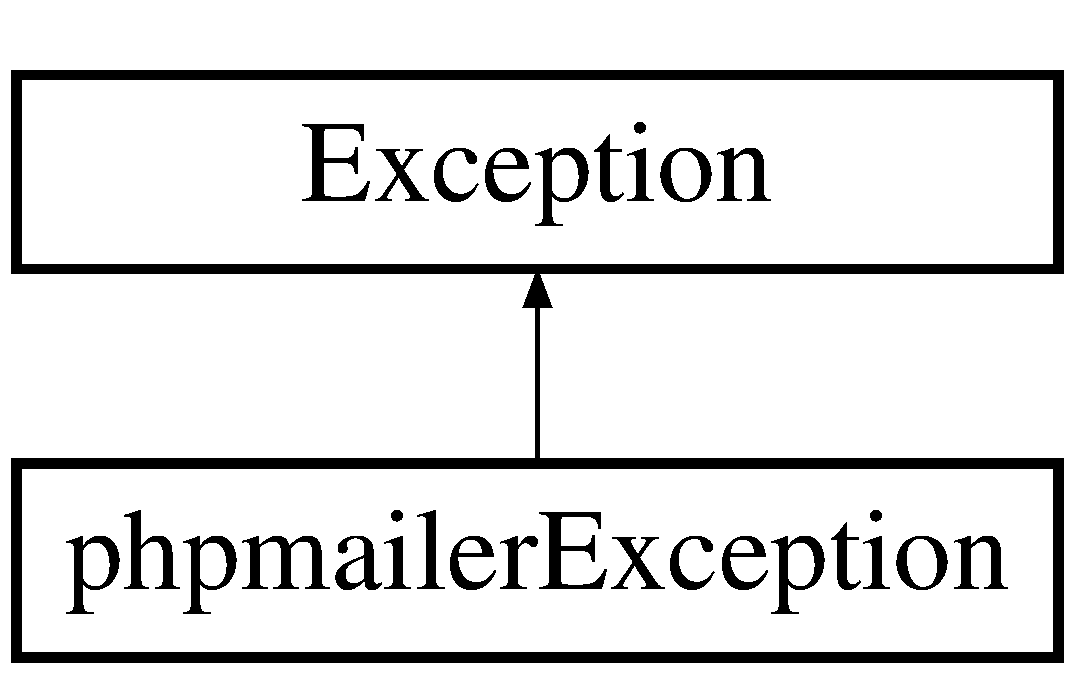
\includegraphics[height=2.000000cm]{classphpmailerException}
\end{center}
\end{figure}
\subsection*{Public 成员函数}
\begin{DoxyCompactItemize}
\item 
\hypertarget{classphpmailerException_aeea8c4a8f2abac4f1ca70c6beb4d356d}{{\bfseries error\+Message} ()}\label{classphpmailerException_aeea8c4a8f2abac4f1ca70c6beb4d356d}

\end{DoxyCompactItemize}


该类的文档由以下文件生成\+:\begin{DoxyCompactItemize}
\item 
framework/lib/vendor/email/P\+H\+P\+Mailer.\+class.\+php\end{DoxyCompactItemize}

\hypertarget{classSession}{\section{Session类 参考}
\label{classSession}\index{Session@{Session}}
}
\subsection*{静态 Public 成员函数}
\begin{DoxyCompactItemize}
\item 
\hypertarget{classSession_a875e07190929d60a64e2bac59f33e33a}{static {\bfseries set} (\$key, \$val)}\label{classSession_a875e07190929d60a64e2bac59f33e33a}

\item 
\hypertarget{classSession_a555ab9c7731c0103b16baf165e34efe8}{static {\bfseries get} (\$key)}\label{classSession_a555ab9c7731c0103b16baf165e34efe8}

\item 
\hypertarget{classSession_a95c5924802a7a671d09e9c3582843938}{static {\bfseries rm} (\$key)}\label{classSession_a95c5924802a7a671d09e9c3582843938}

\item 
\hypertarget{classSession_afa763e91cf165dc4f0e64d2d7a383ecf}{static {\bfseries exist} (\$key)}\label{classSession_afa763e91cf165dc4f0e64d2d7a383ecf}

\item 
\hypertarget{classSession_a4cad41d7bac681f046e92396d59f1603}{static {\bfseries clean} ()}\label{classSession_a4cad41d7bac681f046e92396d59f1603}

\item 
\hypertarget{classSession_a68df91bf431785dd796086d26ce38699}{static {\bfseries expire} (\$min=null)}\label{classSession_a68df91bf431785dd796086d26ce38699}

\item 
\hypertarget{classSession_af336de5d253cd1e891f4c03a9fd614bb}{static {\bfseries sid} (\$id=null)}\label{classSession_af336de5d253cd1e891f4c03a9fd614bb}

\item 
\hypertarget{classSession_a5746f70fe1b29e72108d43d11b96bb90}{static {\bfseries name} (\$name=null)}\label{classSession_a5746f70fe1b29e72108d43d11b96bb90}

\item 
\hypertarget{classSession_a8a9ba8bdd531f9f5617d482705cc6d9e}{static {\bfseries path} (\$path=null)}\label{classSession_a8a9ba8bdd531f9f5617d482705cc6d9e}

\item 
\hypertarget{classSession_ac3f406fa774173d3fdc5df9e2ddd18ed}{static {\bfseries status} ()}\label{classSession_ac3f406fa774173d3fdc5df9e2ddd18ed}

\end{DoxyCompactItemize}


该类的文档由以下文件生成\+:\begin{DoxyCompactItemize}
\item 
framework/kernel/Session.\+class.\+php\end{DoxyCompactItemize}

\hypertarget{classSMTP}{\section{S\+M\+T\+P类 参考}
\label{classSMTP}\index{S\+M\+T\+P@{S\+M\+T\+P}}
}
\subsection*{Public 成员函数}
\begin{DoxyCompactItemize}
\item 
\hyperlink{classSMTP_a943dd07e8b4b4f928b9aa71073939e0f}{\+\_\+\+\_\+construct} ()
\item 
\hyperlink{classSMTP_a8fba663a06f03ca0ffb142d5e4141235}{Connect} (\$host, \$port=0, \$tval=30)
\item 
\hyperlink{classSMTP_a98589ff1441c3c227f6ed12baee8d0cd}{Start\+T\+L\+S} ()
\item 
\hyperlink{classSMTP_a09bed676e22ceb5b30f4b90b0cb8a321}{Authenticate} (\$username, \$password)
\item 
\hyperlink{classSMTP_a1b04ed74ebc02d0e04ab61933ec7089e}{Connected} ()
\item 
\hyperlink{classSMTP_a6a46029fbb02a0bdf9f4680d95589f26}{Close} ()
\item 
\hyperlink{classSMTP_a19b1e3858b6474cace472f85e5dd75e4}{Data} (\$msg\+\_\+data)
\item 
\hyperlink{classSMTP_a497ea40eb9c62b103228a1a4e3b3cdbd}{Hello} (\$host= '')
\item 
\hyperlink{classSMTP_ab1377e8100ab85ecd152992dbcff1990}{Mail} (\$from)
\item 
\hyperlink{classSMTP_a8d7a8c08be60eee2fdb11ace4577eae4}{Quit} (\$close\+\_\+on\+\_\+error=true)
\item 
\hyperlink{classSMTP_abad67dffc11da60d8be10bc1282d8107}{Recipient} (\$to)
\item 
\hyperlink{classSMTP_a32288c4664c4da18c2bde09c558527c3}{Reset} ()
\item 
\hyperlink{classSMTP_adf346869f30d1f09f5437cd0e039f2ca}{Send\+And\+Mail} (\$from)
\item 
\hyperlink{classSMTP_a00e2009833692aa235de5c26b835adc5}{Turn} ()
\item 
\hyperlink{classSMTP_ae69932e8666ab3e15c22ea4d9f03909f}{get\+Error} ()
\end{DoxyCompactItemize}
\subsection*{Public 属性}
\begin{DoxyCompactItemize}
\item 
\hypertarget{classSMTP_ab18d9e6b53ece65286ba6a83af7f9576}{{\bfseries \$\+S\+M\+T\+P\+\_\+\+P\+O\+R\+T} = 25}\label{classSMTP_ab18d9e6b53ece65286ba6a83af7f9576}

\item 
\hypertarget{classSMTP_ab92088467c740f1c76ef8a54c30bd955}{{\bfseries \$\+C\+R\+L\+F} = \char`\"{}\textbackslash{}r\textbackslash{}n\char`\"{}}\label{classSMTP_ab92088467c740f1c76ef8a54c30bd955}

\item 
\hypertarget{classSMTP_aecf5a15107efffb004210746eb3e58bf}{{\bfseries \$do\+\_\+debug}}\label{classSMTP_aecf5a15107efffb004210746eb3e58bf}

\item 
\hypertarget{classSMTP_ac682fd7712ecbd5f11917c99d173de43}{{\bfseries \$do\+\_\+verp} = false}\label{classSMTP_ac682fd7712ecbd5f11917c99d173de43}

\end{DoxyCompactItemize}


\subsection{详细描述}
\hyperlink{classSMTP}{S\+M\+T\+P} is rfc 821 compliant and implements all the rfc 821 \hyperlink{classSMTP}{S\+M\+T\+P} commands except T\+U\+R\+N which will always return a not implemented error. \hyperlink{classSMTP}{S\+M\+T\+P} also provides some utility methods for sending mail to an \hyperlink{classSMTP}{S\+M\+T\+P} server. original author\+: Chris Ryan 

\subsection{构造及析构函数说明}
\hypertarget{classSMTP_a943dd07e8b4b4f928b9aa71073939e0f}{\index{S\+M\+T\+P@{S\+M\+T\+P}!\+\_\+\+\_\+construct@{\+\_\+\+\_\+construct}}
\index{\+\_\+\+\_\+construct@{\+\_\+\+\_\+construct}!S\+M\+T\+P@{S\+M\+T\+P}}
\subsubsection[{\+\_\+\+\_\+construct}]{\setlength{\rightskip}{0pt plus 5cm}S\+M\+T\+P\+::\+\_\+\+\_\+construct (
\begin{DoxyParamCaption}
{}
\end{DoxyParamCaption}
)}}\label{classSMTP_a943dd07e8b4b4f928b9aa71073939e0f}
Initialize the class so that the data is in a known state.  public \begin{DoxyReturn}{返回}
void 
\end{DoxyReturn}


\subsection{成员函数说明}
\hypertarget{classSMTP_a09bed676e22ceb5b30f4b90b0cb8a321}{\index{S\+M\+T\+P@{S\+M\+T\+P}!Authenticate@{Authenticate}}
\index{Authenticate@{Authenticate}!S\+M\+T\+P@{S\+M\+T\+P}}
\subsubsection[{Authenticate}]{\setlength{\rightskip}{0pt plus 5cm}S\+M\+T\+P\+::\+Authenticate (
\begin{DoxyParamCaption}
\item[{}]{\$username, }
\item[{}]{\$password}
\end{DoxyParamCaption}
)}}\label{classSMTP_a09bed676e22ceb5b30f4b90b0cb8a321}
Performs \hyperlink{classSMTP}{S\+M\+T\+P} authentication. Must be run after running the \hyperlink{classSMTP_a497ea40eb9c62b103228a1a4e3b3cdbd}{Hello()} method. Returns true if successfully authenticated.  public \begin{DoxyReturn}{返回}
bool 
\end{DoxyReturn}
\hypertarget{classSMTP_a6a46029fbb02a0bdf9f4680d95589f26}{\index{S\+M\+T\+P@{S\+M\+T\+P}!Close@{Close}}
\index{Close@{Close}!S\+M\+T\+P@{S\+M\+T\+P}}
\subsubsection[{Close}]{\setlength{\rightskip}{0pt plus 5cm}S\+M\+T\+P\+::\+Close (
\begin{DoxyParamCaption}
{}
\end{DoxyParamCaption}
)}}\label{classSMTP_a6a46029fbb02a0bdf9f4680d95589f26}
Closes the socket and cleans up the state of the class. It is not considered good to use this function without first trying to use Q\+U\+I\+T.  public \begin{DoxyReturn}{返回}
void 
\end{DoxyReturn}


参考自 Connected() , 以及 Quit().

\hypertarget{classSMTP_a8fba663a06f03ca0ffb142d5e4141235}{\index{S\+M\+T\+P@{S\+M\+T\+P}!Connect@{Connect}}
\index{Connect@{Connect}!S\+M\+T\+P@{S\+M\+T\+P}}
\subsubsection[{Connect}]{\setlength{\rightskip}{0pt plus 5cm}S\+M\+T\+P\+::\+Connect (
\begin{DoxyParamCaption}
\item[{}]{\$host, }
\item[{}]{\$port = {\ttfamily 0}, }
\item[{}]{\$tval = {\ttfamily 30}}
\end{DoxyParamCaption}
)}}\label{classSMTP_a8fba663a06f03ca0ffb142d5e4141235}
Connect to the server specified on the port specified. If the port is not specified use the default S\+M\+T\+P\+\_\+\+P\+O\+R\+T. If tval is specified then a connection will try and be established with the server for that number of seconds. If tval is not specified the default is 30 seconds to try on the connection.

\hyperlink{classSMTP}{S\+M\+T\+P} C\+O\+D\+E S\+U\+C\+C\+E\+S\+S\+: 220 \hyperlink{classSMTP}{S\+M\+T\+P} C\+O\+D\+E F\+A\+I\+L\+U\+R\+E\+: 421  public \begin{DoxyReturn}{返回}
bool 
\end{DoxyReturn}
\hypertarget{classSMTP_a1b04ed74ebc02d0e04ab61933ec7089e}{\index{S\+M\+T\+P@{S\+M\+T\+P}!Connected@{Connected}}
\index{Connected@{Connected}!S\+M\+T\+P@{S\+M\+T\+P}}
\subsubsection[{Connected}]{\setlength{\rightskip}{0pt plus 5cm}S\+M\+T\+P\+::\+Connected (
\begin{DoxyParamCaption}
{}
\end{DoxyParamCaption}
)}}\label{classSMTP_a1b04ed74ebc02d0e04ab61933ec7089e}
Returns true if connected to a server otherwise false  public \begin{DoxyReturn}{返回}
bool 
\end{DoxyReturn}
\hypertarget{classSMTP_a19b1e3858b6474cace472f85e5dd75e4}{\index{S\+M\+T\+P@{S\+M\+T\+P}!Data@{Data}}
\index{Data@{Data}!S\+M\+T\+P@{S\+M\+T\+P}}
\subsubsection[{Data}]{\setlength{\rightskip}{0pt plus 5cm}S\+M\+T\+P\+::\+Data (
\begin{DoxyParamCaption}
\item[{}]{\$msg\+\_\+data}
\end{DoxyParamCaption}
)}}\label{classSMTP_a19b1e3858b6474cace472f85e5dd75e4}
Issues a data command and sends the msg\+\_\+data to the server finializing the mail transaction. \$msg\+\_\+data is the message that is to be send with the headers. Each header needs to be on a single line followed by a $<$\+C\+R\+L\+F$>$ with the message headers and the message body being seperated by and additional $<$\+C\+R\+L\+F$>$.

Implements rfc 821\+: D\+A\+T\+A $<$\+C\+R\+L\+F$>$

\hyperlink{classSMTP}{S\+M\+T\+P} C\+O\+D\+E I\+N\+T\+E\+R\+M\+E\+D\+I\+A\+T\+E\+: 354 \mbox{[}data\mbox{]} $<$\+C\+R\+L\+F$>$.$<$\+C\+R\+L\+F$>$ \hyperlink{classSMTP}{S\+M\+T\+P} C\+O\+D\+E S\+U\+C\+C\+E\+S\+S\+: 250 \hyperlink{classSMTP}{S\+M\+T\+P} C\+O\+D\+E F\+A\+I\+L\+U\+R\+E\+: 552,554,451,452 \hyperlink{classSMTP}{S\+M\+T\+P} C\+O\+D\+E F\+A\+I\+L\+U\+R\+E\+: 451,554 \hyperlink{classSMTP}{S\+M\+T\+P} C\+O\+D\+E E\+R\+R\+O\+R \+: 500,501,503,421  public \begin{DoxyReturn}{返回}
bool 
\end{DoxyReturn}
\hypertarget{classSMTP_ae69932e8666ab3e15c22ea4d9f03909f}{\index{S\+M\+T\+P@{S\+M\+T\+P}!get\+Error@{get\+Error}}
\index{get\+Error@{get\+Error}!S\+M\+T\+P@{S\+M\+T\+P}}
\subsubsection[{get\+Error}]{\setlength{\rightskip}{0pt plus 5cm}S\+M\+T\+P\+::get\+Error (
\begin{DoxyParamCaption}
{}
\end{DoxyParamCaption}
)}}\label{classSMTP_ae69932e8666ab3e15c22ea4d9f03909f}
Get the current error  public \begin{DoxyReturn}{返回}
array 
\end{DoxyReturn}
\hypertarget{classSMTP_a497ea40eb9c62b103228a1a4e3b3cdbd}{\index{S\+M\+T\+P@{S\+M\+T\+P}!Hello@{Hello}}
\index{Hello@{Hello}!S\+M\+T\+P@{S\+M\+T\+P}}
\subsubsection[{Hello}]{\setlength{\rightskip}{0pt plus 5cm}S\+M\+T\+P\+::\+Hello (
\begin{DoxyParamCaption}
\item[{}]{\$host = {\ttfamily ''}}
\end{DoxyParamCaption}
)}}\label{classSMTP_a497ea40eb9c62b103228a1a4e3b3cdbd}
Sends the H\+E\+L\+O command to the smtp server. This makes sure that we and the server are in the same known state.

Implements from rfc 821\+: H\+E\+L\+O $<$\+S\+P$>$ $<$domain$>$ $<$\+C\+R\+L\+F$>$

\hyperlink{classSMTP}{S\+M\+T\+P} C\+O\+D\+E S\+U\+C\+C\+E\+S\+S\+: 250 \hyperlink{classSMTP}{S\+M\+T\+P} C\+O\+D\+E E\+R\+R\+O\+R \+: 500, 501, 504, 421  public \begin{DoxyReturn}{返回}
bool 
\end{DoxyReturn}
\hypertarget{classSMTP_ab1377e8100ab85ecd152992dbcff1990}{\index{S\+M\+T\+P@{S\+M\+T\+P}!Mail@{Mail}}
\index{Mail@{Mail}!S\+M\+T\+P@{S\+M\+T\+P}}
\subsubsection[{Mail}]{\setlength{\rightskip}{0pt plus 5cm}S\+M\+T\+P\+::\+Mail (
\begin{DoxyParamCaption}
\item[{}]{\$from}
\end{DoxyParamCaption}
)}}\label{classSMTP_ab1377e8100ab85ecd152992dbcff1990}
Starts a mail transaction from the email address specified in \$from. Returns true if successful or false otherwise. If True the mail transaction is started and then one or more Recipient commands may be called followed by a Data command.

Implements rfc 821\+: M\+A\+I\+L $<$\+S\+P$>$ F\+R\+O\+M\+:$<$reverse-\/path$>$ $<$\+C\+R\+L\+F$>$

\hyperlink{classSMTP}{S\+M\+T\+P} C\+O\+D\+E S\+U\+C\+C\+E\+S\+S\+: 250 \hyperlink{classSMTP}{S\+M\+T\+P} C\+O\+D\+E S\+U\+C\+C\+E\+S\+S\+: 552,451,452 \hyperlink{classSMTP}{S\+M\+T\+P} C\+O\+D\+E S\+U\+C\+C\+E\+S\+S\+: 500,501,421  public \begin{DoxyReturn}{返回}
bool 
\end{DoxyReturn}
\hypertarget{classSMTP_a8d7a8c08be60eee2fdb11ace4577eae4}{\index{S\+M\+T\+P@{S\+M\+T\+P}!Quit@{Quit}}
\index{Quit@{Quit}!S\+M\+T\+P@{S\+M\+T\+P}}
\subsubsection[{Quit}]{\setlength{\rightskip}{0pt plus 5cm}S\+M\+T\+P\+::\+Quit (
\begin{DoxyParamCaption}
\item[{}]{\$close\+\_\+on\+\_\+error = {\ttfamily true}}
\end{DoxyParamCaption}
)}}\label{classSMTP_a8d7a8c08be60eee2fdb11ace4577eae4}
Sends the quit command to the server and then closes the socket if there is no error or the \$close\+\_\+on\+\_\+error argument is true.

Implements from rfc 821\+: Q\+U\+I\+T $<$\+C\+R\+L\+F$>$

\hyperlink{classSMTP}{S\+M\+T\+P} C\+O\+D\+E S\+U\+C\+C\+E\+S\+S\+: 221 \hyperlink{classSMTP}{S\+M\+T\+P} C\+O\+D\+E E\+R\+R\+O\+R \+: 500  public \begin{DoxyReturn}{返回}
bool 
\end{DoxyReturn}
\hypertarget{classSMTP_abad67dffc11da60d8be10bc1282d8107}{\index{S\+M\+T\+P@{S\+M\+T\+P}!Recipient@{Recipient}}
\index{Recipient@{Recipient}!S\+M\+T\+P@{S\+M\+T\+P}}
\subsubsection[{Recipient}]{\setlength{\rightskip}{0pt plus 5cm}S\+M\+T\+P\+::\+Recipient (
\begin{DoxyParamCaption}
\item[{}]{\$to}
\end{DoxyParamCaption}
)}}\label{classSMTP_abad67dffc11da60d8be10bc1282d8107}
Sends the command R\+C\+P\+T to the \hyperlink{classSMTP}{S\+M\+T\+P} server with the T\+O\+: argument of \$to. Returns true if the recipient was accepted false if it was rejected.

Implements from rfc 821\+: R\+C\+P\+T $<$\+S\+P$>$ T\+O\+:$<$forward-\/path$>$ $<$\+C\+R\+L\+F$>$

\hyperlink{classSMTP}{S\+M\+T\+P} C\+O\+D\+E S\+U\+C\+C\+E\+S\+S\+: 250,251 \hyperlink{classSMTP}{S\+M\+T\+P} C\+O\+D\+E F\+A\+I\+L\+U\+R\+E\+: 550,551,552,553,450,451,452 \hyperlink{classSMTP}{S\+M\+T\+P} C\+O\+D\+E E\+R\+R\+O\+R \+: 500,501,503,421  public \begin{DoxyReturn}{返回}
bool 
\end{DoxyReturn}
\hypertarget{classSMTP_a32288c4664c4da18c2bde09c558527c3}{\index{S\+M\+T\+P@{S\+M\+T\+P}!Reset@{Reset}}
\index{Reset@{Reset}!S\+M\+T\+P@{S\+M\+T\+P}}
\subsubsection[{Reset}]{\setlength{\rightskip}{0pt plus 5cm}S\+M\+T\+P\+::\+Reset (
\begin{DoxyParamCaption}
{}
\end{DoxyParamCaption}
)}}\label{classSMTP_a32288c4664c4da18c2bde09c558527c3}
Sends the R\+S\+E\+T command to abort and transaction that is currently in progress. Returns true if successful false otherwise.

Implements rfc 821\+: R\+S\+E\+T $<$\+C\+R\+L\+F$>$

\hyperlink{classSMTP}{S\+M\+T\+P} C\+O\+D\+E S\+U\+C\+C\+E\+S\+S\+: 250 \hyperlink{classSMTP}{S\+M\+T\+P} C\+O\+D\+E E\+R\+R\+O\+R \+: 500,501,504,421  public \begin{DoxyReturn}{返回}
bool 
\end{DoxyReturn}
\hypertarget{classSMTP_adf346869f30d1f09f5437cd0e039f2ca}{\index{S\+M\+T\+P@{S\+M\+T\+P}!Send\+And\+Mail@{Send\+And\+Mail}}
\index{Send\+And\+Mail@{Send\+And\+Mail}!S\+M\+T\+P@{S\+M\+T\+P}}
\subsubsection[{Send\+And\+Mail}]{\setlength{\rightskip}{0pt plus 5cm}S\+M\+T\+P\+::\+Send\+And\+Mail (
\begin{DoxyParamCaption}
\item[{}]{\$from}
\end{DoxyParamCaption}
)}}\label{classSMTP_adf346869f30d1f09f5437cd0e039f2ca}
Starts a mail transaction from the email address specified in \$from. Returns true if successful or false otherwise. If True the mail transaction is started and then one or more Recipient commands may be called followed by a Data command. This command will send the message to the users terminal if they are logged in and send them an email.

Implements rfc 821\+: S\+A\+M\+L $<$\+S\+P$>$ F\+R\+O\+M\+:$<$reverse-\/path$>$ $<$\+C\+R\+L\+F$>$

\hyperlink{classSMTP}{S\+M\+T\+P} C\+O\+D\+E S\+U\+C\+C\+E\+S\+S\+: 250 \hyperlink{classSMTP}{S\+M\+T\+P} C\+O\+D\+E S\+U\+C\+C\+E\+S\+S\+: 552,451,452 \hyperlink{classSMTP}{S\+M\+T\+P} C\+O\+D\+E S\+U\+C\+C\+E\+S\+S\+: 500,501,502,421  public \begin{DoxyReturn}{返回}
bool 
\end{DoxyReturn}
\hypertarget{classSMTP_a98589ff1441c3c227f6ed12baee8d0cd}{\index{S\+M\+T\+P@{S\+M\+T\+P}!Start\+T\+L\+S@{Start\+T\+L\+S}}
\index{Start\+T\+L\+S@{Start\+T\+L\+S}!S\+M\+T\+P@{S\+M\+T\+P}}
\subsubsection[{Start\+T\+L\+S}]{\setlength{\rightskip}{0pt plus 5cm}S\+M\+T\+P\+::\+Start\+T\+L\+S (
\begin{DoxyParamCaption}
{}
\end{DoxyParamCaption}
)}}\label{classSMTP_a98589ff1441c3c227f6ed12baee8d0cd}
Initiate a T\+L\+S communication with the server.

\hyperlink{classSMTP}{S\+M\+T\+P} C\+O\+D\+E 220 Ready to start T\+L\+S \hyperlink{classSMTP}{S\+M\+T\+P} C\+O\+D\+E 501 Syntax error (no parameters allowed) \hyperlink{classSMTP}{S\+M\+T\+P} C\+O\+D\+E 454 T\+L\+S not available due to temporary reason  public \begin{DoxyReturn}{返回}
bool success 
\end{DoxyReturn}
\hypertarget{classSMTP_a00e2009833692aa235de5c26b835adc5}{\index{S\+M\+T\+P@{S\+M\+T\+P}!Turn@{Turn}}
\index{Turn@{Turn}!S\+M\+T\+P@{S\+M\+T\+P}}
\subsubsection[{Turn}]{\setlength{\rightskip}{0pt plus 5cm}S\+M\+T\+P\+::\+Turn (
\begin{DoxyParamCaption}
{}
\end{DoxyParamCaption}
)}}\label{classSMTP_a00e2009833692aa235de5c26b835adc5}
This is an optional command for \hyperlink{classSMTP}{S\+M\+T\+P} that this class does not support. This method is here to make the R\+F\+C821 Definition complete for this class and {\bfseries may} be implimented in the future

Implements from rfc 821\+: T\+U\+R\+N $<$\+C\+R\+L\+F$>$

\hyperlink{classSMTP}{S\+M\+T\+P} C\+O\+D\+E S\+U\+C\+C\+E\+S\+S\+: 250 \hyperlink{classSMTP}{S\+M\+T\+P} C\+O\+D\+E F\+A\+I\+L\+U\+R\+E\+: 502 \hyperlink{classSMTP}{S\+M\+T\+P} C\+O\+D\+E E\+R\+R\+O\+R \+: 500, 503  public \begin{DoxyReturn}{返回}
bool 
\end{DoxyReturn}


该类的文档由以下文件生成\+:\begin{DoxyCompactItemize}
\item 
framework/lib/vendor/email/S\+M\+T\+P.\+class.\+php\end{DoxyCompactItemize}

\hypertarget{classUpload}{\section{Upload类 参考}
\label{classUpload}\index{Upload@{Upload}}
}
\subsection*{Public 成员函数}
\begin{DoxyCompactItemize}
\item 
\hypertarget{classUpload_acc3501937980700dd62cd997d12cd94b}{{\bfseries \+\_\+\+\_\+construct} (\$type= 'images', \$ext\+Arr=array('jpg', 'gif', 'png'))}\label{classUpload_acc3501937980700dd62cd997d12cd94b}

\item 
\hypertarget{classUpload_ae3c33e8a28fcb3ded1743dc67ef4d4fc}{{\bfseries upload} (\$name= 'file')}\label{classUpload_ae3c33e8a28fcb3ded1743dc67ef4d4fc}

\end{DoxyCompactItemize}


该类的文档由以下文件生成\+:\begin{DoxyCompactItemize}
\item 
framework/lib/core/Upload.\+class.\+php\end{DoxyCompactItemize}

%--- End generated contents ---

% Index
\newpage
\phantomsection
\addcontentsline{toc}{chapter}{索引}
\printindex

\end{document}
